\chapter{Análisis Funcional}

\section{Actores}
\label{analysis:actors}
En el software desarrollado, cada rol dentro del staff de RVA ha sido considerado como un actor diferente. Para el contexto del presente proyecto, el cargo de cada actor corresponde a su nombre, lo que quiere decir que si un actor lleva por nombre ''Administrador'', se entenderá que su cargo es ''Administrador de la comunidad de RVA''. Sólo los jugadores no cuentan con un cargo dentro de RVA.

La especificación de todos los actores se puede encontrar a continuación en la \autoref{table:analysis:actors}.

\begin{center}
  \begin{tabular}{| p{3cm} | p{4.5cm} | p{4.5cm} | p{2cm} |}
    \hline
    \multicolumn{4}{|c|}{\textbf{Actores}} \\
    \hline
    \multicolumn{1}{|c|}{\textbf{Actor}} & \multicolumn{1}{|c|}{\textbf{Función}} & \multicolumn{1}{|c|}{\textbf{Conocimientos}} & \multicolumn{1}{|c|}{\textbf{Privilegio}}\\
    \hline
    {\textbf{Administrador}} & Cumple con todas las funciones dentro de la comunidad como mantener autos, pistas, sesiones y manejo general del software. Configura el software para el resto de los usuarios. & Requiere conocimiento sobre como funciona el sistema en su totalidad, comprendiendo también el contexto en el que funciona RVA como comunidad. & Máximo. \\ \hline
    {\textbf{Organizador}} & Cumple con funciones específicamente relacionadas al manejo de sesiones multijugador y el procesamiento de los puntajes. & Requiere conocimiento específico de como subir archivos de sesión a la aplicación web, y un contexto general de como funciona RVA. & Intermedio (módulo de sesiones).\\ \hline
    {\textbf{Moderador}} & Utiliza las funciones específicas de manejo de usuarios, tal como la edición de perfiles o aplicación de infracciones. & Requiere conocimientos que se limitan al manejo de usuarios dentro de la web. & Intermedio (manejo de usuarios).\\ \hline
    {\textbf{Jugador}} & Utiliza la página sólo para visualizar la información que esta ofrece. & No requiere conocimientos técnicos más allá de iniciar sesión. & Ninguno.\\ \hline
  \end{tabular}
  \captionof{table}{Tabla de actores}\label{table:analysis:actors}
\end{center}

\newpage

\section{Casos de Uso}
Esta sección contiene todos los diagramas de casos de uso relevantes para el proyecto, los cuales vienen ilustrados en las \cref{fig:privileges_module,fig:rva_cars_module_1,fig:rva_cars_module_2,fig:rva_tracks_module_1,fig:rva_tracks_module_2,fig:rva_seasons_module_1,fig:rva_seasons_module_2,fig:rva_sessions_module_1,fig:rva_sessions_module_2}. Todos los casos de uso contarán con su respectiva especificación y detalle según corresponda.

\subsection{Diagramas de Casos de Uso}
\label{analysis:usecases}

\begin{figure}[H]
  \begin{center}
    \includegraphics{privileges_module.png}
  \end{center}
  \caption[Diagrama de casos de uso del módulo de privilegios]{Diagrama de  casos de uso del módulo de privilegios}
  \label{fig:privileges_module}
\end{figure}

\begin{figure}[H]
  \begin{center}
    \includegraphics{rva_cars_module_1.png}
  \end{center}
  \caption[Primer diagrama de casos de uso  del módulo de autos]{Primer diagrama de casos de uso del módulo de autos}
  \label{fig:rva_cars_module_1}
\end{figure}

\begin{figure}[H]
  \begin{center}
    \includegraphics{rva_cars_module_2.png}
  \end{center}
  \caption[Segundo diagrama de casos de uso del módulo de autos]{Segundo diagrama de casos de uso del módulo de autos}
  \label{fig:rva_cars_module_2}
\end{figure}

\begin{figure}[H]
  \begin{center}
    \includegraphics{rva_tracks_module_1.png}
  \end{center}
  \caption[Primer diagrama de casos de uso del módulo de pistas]{Primer diagrama de casos de uso del módulo de pistas}
  \label{fig:rva_tracks_module_1}
\end{figure}

\begin{figure}[H]
  \begin{center}
    \includegraphics{rva_tracks_module_2.png}
  \end{center}
  \caption[Segundo diagrama de casos de uso del módulo de pistas]{Segundo diagrama de casos de uso del módulo de pistas}
  \label{fig:rva_tracks_module_2}
\end{figure}

\begin{figure}[H]
  \begin{center}
    \includegraphics{rva_seasons_module_1.png}
  \end{center}
  \caption[Primer diagrama de casos de uso del módulo de temporadas]{Primer diagrama de casos de uso del módulo de temporadas}
  \label{fig:rva_seasons_module_1}
\end{figure}

\begin{figure}[H]
  \begin{center}
    \includegraphics{rva_seasons_module_2.png}
  \end{center}
  \caption[Segundo diagrama de casos de uso del módulo de temporadas]{Segundo diagrama de casos de uso del módulo de temporadas}
  \label{fig:rva_seasons_module_2}
\end{figure}

\begin{figure}[H]
  \begin{center}
    \includegraphics{rva_sessions_module_1.png}
  \end{center}
  \caption[Primer diagrama de casos de uso del módulo de sesiones]{Primer diagrama de casos de uso del módulo de sesiones}
  \label{fig:rva_sessions_module_1}
\end{figure}

\begin{figure}[H]
  \begin{center}
    \includegraphics{rva_sessions_module_2.png}
  \end{center}
  \caption[Segundo diagrama de casos de uso del módulo de sesiones]{Segundo diagrama de casos de uso del módulo de sesiones}
  \label{fig:rva_sessions_module_2}
\end{figure}

\newpage

\subsection{Especificación de los Casos de Uso}
\label{analysis:usecases:specification}
En esta sección se detallan todos los casos de uso diagramados en la \autoref{analysis:usecases}. De acuerdo con la jerarquía de actores presentada en la \autoref{analysis:actors}, se entenderá que, si un actor de tipo ''Jugador'' puede realizar una acción específica, entonces cualquier otro de los actores con cargo podrá realizarla también.

A continuación, la \autoref{table:usecase:specification} contiene los nombres y actores asociados a cada uno de los diagramas de casos de uso. Los casos de uso cuyos actores y nombre han sido marcados en negrita serán detallados posteriormente.

\begin{center}
  \begin{tabular}{| p{1.5cm} | p{6.5cm} | p{5.5cm} |}
    \hline
    \multicolumn{3}{|c|}{\textbf{Casos de Uso}} \\
    \hline
    \multicolumn{1}{|c|}{\textbf{Id}} & \multicolumn{1}{|c|}{\textbf{Actor}} & \multicolumn{1}{|c|}{\textbf{Nombre}}\\
    \hline
    
    % Módulo de Privilegios
    {\textbf{CU\_01}} & \textbf{Administrador, Moderador, Organizador y Jugador} & \textbf{Iniciar Sesión}\\ \hline
    
    % Módulo de Autos
    {\textbf{CU\_02}} & \textbf{Administrador} & \textbf{Importar Autos}\\ \hline
    {\textbf{CU\_03}} & Administrador & Crear Auto\\ \hline
    {\textbf{CU\_04}} & Administrador & Editar Auto \\\hline
    {\textbf{CU\_05}} & Administrador & Eliminar Auto\\ \hline
    {\textbf{CU\_06}} & Administrador & Validar Archivo CSV\\ \hline
    {\textbf{CU\_07}} & Administrador & Validar Parámetros\\ \hline
    
    {\textbf{CU\_08}} & Jugador & Visualizar Autos\\ \hline
    {\textbf{CU\_09}} & \textbf{Jugador} & \textbf{Visualizar un Auto}\\ \hline
    {\textbf{CU\_10}} & Jugador & Filtrar por Categoría\\ \hline
    
    % Módulo de Pistas
    {\textbf{CU\_11}} & \textbf{Administrador} & \textbf{Importar Pistas}\\ \hline
    {\textbf{CU\_12}} & Administrador & Crear Pista\\ \hline
    {\textbf{CU\_13}} & Administrador & Editar Pista\\\hline
    {\textbf{CU\_14}} & Administrador & Eliminar Pista\\ \hline
    {\textbf{CU\_15}} & Administrador & Validar Archivo CSV\\ \hline
    {\textbf{CU\_16}} & Administrador & Validar Parámetros\\ \hline
    
    {\textbf{CU\_17}} & Jugador & Visualizar Pistas\\ \hline
    {\textbf{CU\_18}} & Jugador & Visualizar una Pista\\ \hline
    {\textbf{CU\_19}} & Jugador & Filtrar por Temporada\\ \hline
    
    % Módulo de Temporadas
    {\textbf{CU\_20}} & \textbf{Administrador} & \textbf{Crear Temporada}\\ \hline
    {\textbf{CU\_21}} & \textbf{Administrador} & \textbf{Eliminar Temporada}\\ \hline
    {\textbf{CU\_22}} & Administrador & Validar Parámetros\\\hline
    {\textbf{CU\_23}} & Administrador & Crear Rankings Asociados\\ \hline
    {\textbf{CU\_24}} & Administrador & Eliminar Rankings Asociados\\ \hline
    {\textbf{CU\_25}} & Administrador & Eliminar Sesiones Asociadas\\ \hline
    
    {\textbf{CU\_26}} & Jugador & Visualizar Temporadas\\ \hline
    {\textbf{CU\_27}} & Jugador & Visualizar una Temporada\\ \hline
    {\textbf{CU\_28}} & Jugador & Visualizar Ranking\\ \hline
    {\textbf{CU\_29}} & Jugador & Mostrar Tabla de Resultados\\ \hline
    
    % Módulo de Sesiones
    {\textbf{CU\_30}} & \textbf{Administrador y Organizador} & \textbf{Importar Sesión}\\ \hline
    {\textbf{CU\_31}} & Administrador y Organizador & Crear Sesión\\ \hline
    {\textbf{CU\_32}} & \textbf{Administrador y Organizador} & \textbf{Eliminar Sesión}\\ \hline
    {\textbf{CU\_33}} & Administrador y Organizador & Validar Archivo CSV\\ \hline
    {\textbf{CU\_34}} & Administrador y Organizador & Validar Parámetros\\ \hline
    {\textbf{CU\_35}} & Administrador y Organizador & Calcular Resultados\\ \hline
    
    {\textbf{CU\_36}} & Jugador & Visualizar Sesiones\\ \hline
    {\textbf{CU\_37}} & \textbf{Jugador} & \textbf{Visualizar una Sesión}\\ \hline
    {\textbf{CU\_38}} & Jugador & Visualizar Sesiones Recientes\\ \hline
  \end{tabular}
  
  \captionof{table}{Tabla de especificación de casos de uso}\label{table:usecase:specification}
\end{center}

\subsection{Detalle de los Casos de Uso}
A continuación, se presentan tablas de detalle para los casos de uso listados en la \autoref{analysis:usecases:specification} que fueron marcados en negrita. Estos casos de uso también contarán con un detalle de su flujo de eventos básico.

Los casos de uso seleccionados para ser detallados fueron elegidos porque cumplen funciones fundamentales de los requisitos funcionales de la aplicación desarrollada. El resto de los casos de uso solamente contarán con sus precondiciones y una descripción simple.

De acuerdo con lo mencionado anteriormente, las \cref{table:usecase:1,table:usecase:2,table:usecase:9,table:usecase:11,table:usecase:20,table:usecase:21,table:usecase:30,table:usecase:32,table:usecase:37} describen el detalle completo de los casos de uso marcados en negrita en la \autoref{table:usecase:specification}. Las \cref{table:usecase:3,table:usecase:4,table:usecase:5,table:usecase:6,table:usecase:7,table:usecase:8,table:usecase:10,table:usecase:12,table:usecase:13,table:usecase:14,table:usecase:15,table:usecase:16,table:usecase:17,table:usecase:18,table:usecase:19,table:usecase:22,table:usecase:23,table:usecase:24,table:usecase:25,table:usecase:26,table:usecase:27,table:usecase:28,table:usecase:29,table:usecase:31,table:usecase:33,table:usecase:34,table:usecase:35,table:usecase:36,table:usecase:38} describen todos los demás casos de uso.

%
% Privilegios
%

\begin{center}
  \begin{tabular}{| p{7.5cm} | p{7.5cm} |}
    \hline
    \multicolumn{2}{|p{15cm}|}{\textbf{CU\_01\_INICIAR\_SESION} (Usuario)} \\ \hline
    \multicolumn{2}{|p{15cm}|}{\textbf{Pre-Condiciones:} El usuario debe estar en la página web. El usuario debe haberse registrado en la plataforma.} \\ \hline
    \multicolumn{2}{|p{15cm}|}{\textbf{Post-Condiciones:} El usuario inicia sesión en la plataforma.} \\ \hline
    \multicolumn{2}{|p{7.5cm}|}{\textbf{Flujo de Eventos Básicos}} \\ \hline
    \multicolumn{1}{|p{7.5cm}|}{\textbf{Usuarios:} Administrador, Organizador, Moderador y Jugador} & \multicolumn{1}{|p{7.5cm}|}{\textbf{Sistema}} \\ \hline
    
    \multicolumn{1}{|p{7.5cm}|}{} & 
    \multicolumn{1}{|p{7.5cm}|}{1. Renderiza la pantalla de inicio de sesión.}\\ \hline
    
    \multicolumn{1}{|p{7.5cm}|}{2. Ingresa su correo y contraseña, y luego pulsa el botón para iniciar sesión.}& 
    \multicolumn{1}{|p{7.5cm}|}{3. Valida la información ingresada por el usuario.}\\ \hline
    
    \multicolumn{1}{|p{7.5cm}|}{} & 
    \multicolumn{1}{|p{7.5cm}|}{4. Sesión iniciada. Redirecciona al usuario a la página principal.}\\ \hline
    
    \multicolumn{2}{|p{7.5cm}|}{\textbf{Flujo de Eventos Alternativo}} \\ \hline
    
    \multicolumn{1}{|p{7.5cm}|}{\textbf{Usuarios:} Administrador, Organizador, Moderador y Jugador} & \multicolumn{1}{|p{7.5cm}|}{\textbf{Sistema}} \\ \hline
    
    \multicolumn{1}{|p{7.5cm}|}{} & 
    \multicolumn{1}{|p{7.5cm}|}{3 (b). Si las credenciales son incorrectas, el sistema muestra un mensaje de error.}\\ \hline
    
    \multicolumn{1}{|p{7.5cm}|}{} & 
    \multicolumn{1}{|p{7.5cm}|}{4 (b). Vuelve al paso 2 del flujo básico.}\\ \hline
  \end{tabular}
  
  \captionof{table}{Tabla del caso de uso CU\_01\_INICIAR\_SESION}\label{table:usecase:1}
\end{center}

%
% Autos
%

\begin{center}
  \begin{tabular}{| p{7.5cm} | p{7.5cm} |}
    \hline
    \multicolumn{2}{|p{15cm}|}{\textbf{CU\_02\_IMPORTAR\_AUTOS} (Administrador)} \\ \hline
    \multicolumn{2}{|p{15cm}|}{\textbf{Pre-Condiciones:} El administrador debe haber iniciado sesión con sus credenciales.} \\ \hline
    \multicolumn{2}{|p{15cm}|}{\textbf{Post-Condiciones:} El sistema crea los autos y los guarda en la base de datos.} \\ \hline
    \multicolumn{2}{|p{7.5cm}|}{\textbf{Flujo de Eventos Básicos}} \\ \hline
    \multicolumn{1}{|p{7.5cm}|}{\textbf{Usuario:} Administrador} & \multicolumn{1}{|p{7.5cm}|}{\textbf{Sistema}} \\ \hline
    
    \multicolumn{1}{|p{7.5cm}|}{} & 
    \multicolumn{1}{|p{7.5cm}|}{1. Renderiza el formulario de importación de autos.}\\ \hline
    
    \multicolumn{1}{|p{7.5cm}|}{2. Selecciona el archivo CSV con la información de los autos y la temporada. Luego pulsa el botón para importar.}& 
    \multicolumn{1}{|p{7.5cm}|}{}\\ \hline
    
    \multicolumn{1}{|p{7.5cm}|}{}& 
    \multicolumn{1}{|p{7.5cm}|}{3. Llama al \textbf{CU\_06\_VALIDAR\_ARCHIVO\_CSV}.}\\ \hline
    
    \multicolumn{1}{|p{7.5cm}|}{} & 
    \multicolumn{1}{|p{7.5cm}|}{4. El sistema crea las colecciones y las almacena en la base de datos. Se notifica éxito al usuario.}\\ \hline
    
    \multicolumn{2}{|p{7.5cm}|}{\textbf{Flujo de Eventos Alternativo}} \\ \hline
    
    \multicolumn{1}{|p{7.5cm}|}{\textbf{Usuario:} Administrador} & \multicolumn{1}{|p{7.5cm}|}{\textbf{Sistema}} \\ \hline
    
    \multicolumn{1}{|p{7.5cm}|}{} & 
    \multicolumn{1}{|p{7.5cm}|}{3 (b). Si el archivo seleccionado no es válido, el sistema muestra un mensaje de error.}\\ \hline
    
    \multicolumn{1}{|p{7.5cm}|}{} & 
    \multicolumn{1}{|p{7.5cm}|}{4 (b). Vuelve al paso 2 del flujo básico.}\\ \hline
  \end{tabular}
  
  \captionof{table}{Tabla del caso de uso CU\_02\_IMPORTAR\_AUTOS}\label{table:usecase:2}
\end{center}

\begin{center}
  \begin{tabular}{| p{7.5cm} | p{7.5cm} |}
    \hline
    \multicolumn{2}{|p{15cm}|}{\textbf{CU\_03\_CREAR\_AUTO} (Administrador)} \\ \hline
    \multicolumn{2}{|p{15cm}|}{\textbf{Pre-Condiciones:} El administrador debe haber iniciado sesión con sus credenciales.} \\ \hline
    \multicolumn{2}{|p{15cm}|}{\textbf{Descripción:} El sistema guarda el modelo de auto en la base de datos con los datos ingresados por el administrador. } \\
    \hline
  \end{tabular}
  
  \captionof{table}{Tabla del caso de uso CU\_03\_CREAR\_AUTO}\label{table:usecase:3}
\end{center}

\begin{center}
  \begin{tabular}{| p{7.5cm} | p{7.5cm} |}
    \hline
    \multicolumn{2}{|p{15cm}|}{\textbf{CU\_04\_EDITAR\_AUTO} (Administrador)} \\ \hline
    \multicolumn{2}{|p{15cm}|}{\textbf{Pre-Condiciones:} El administrador debe haber iniciado sesión con sus credenciales.} \\ \hline
    \multicolumn{2}{|p{15cm}|}{\textbf{Descripción:} El sistema actualiza el modelo de auto en la base de datos con los datos ingresados por el administrador.} \\
    \hline
  \end{tabular}
  
  \captionof{table}{Tabla del caso de uso CU\_04\_EDITAR\_AUTO}\label{table:usecase:4}
\end{center}

\begin{center}
  \begin{tabular}{| p{7.5cm} | p{7.5cm} |}
    \hline
    \multicolumn{2}{|p{15cm}|}{\textbf{CU\_05\_ELIMINAR\_AUTO} (Administrador)} \\ \hline
    \multicolumn{2}{|p{15cm}|}{\textbf{Pre-Condiciones:} El administrador debe haber iniciado sesión con sus credenciales.} \\ \hline
    \multicolumn{2}{|p{15cm}|}{\textbf{Descripción:} El sistema elimina el modelo de auto en la base de datos.} \\
    \hline
  \end{tabular}
  
  \captionof{table}{Tabla del caso de uso CU\_05\_ELIMINAR\_AUTO}\label{table:usecase:5}
\end{center}

\begin{center}
  \begin{tabular}{| p{7.5cm} | p{7.5cm} |}
    \hline
    \multicolumn{2}{|p{15cm}|}{\textbf{CU\_06\_VALIDAR\_ARCHIVO\_CSV}} \\ \hline
    \multicolumn{2}{|p{15cm}|}{\textbf{Pre-Condiciones:} Debe ser activado por \textbf{CU\_02}.} \\ \hline
    \multicolumn{2}{|p{15cm}|}{\textbf{Descripción:} El sistema lee el archivo y verifica que éste esté en el formato adecuado, y que contenga datos válidos para crear modelos de autos.} \\
    \hline
  \end{tabular}
  
  \captionof{table}{Tabla del caso de uso CU\_06\_VALIDAR\_ARCHIVO\_CSV}\label{table:usecase:6}
\end{center}

\begin{center}
  \begin{tabular}{| p{7.5cm} | p{7.5cm} |}
    \hline
    \multicolumn{2}{|p{15cm}|}{\textbf{CU\_07\_VALIDAR\_PARAMETROS}} \\ \hline
    \multicolumn{2}{|p{15cm}|}{\textbf{Pre-Condiciones:} Debe ser activado por \textbf{CU\_03}.} \\ \hline
    \multicolumn{2}{|p{15cm}|}{\textbf{Descripción:} Verifica que los parámetros cumplan con las restricciones del modelo de auto.} \\
    \hline
  \end{tabular}
  
  \captionof{table}{Tabla del caso de uso CU\_07\_VALIDAR\_PARAMETROS}\label{table:usecase:7}
\end{center}

\begin{center}
  \begin{tabular}{| p{7.5cm} | p{7.5cm} |}
    \hline
    \multicolumn{2}{|p{15cm}|}{\textbf{CU\_08\_VISUALIZAR\_AUTOS} (Jugador)} \\ \hline
    \multicolumn{2}{|p{15cm}|}{\textbf{Pre-Condiciones:} No tiene.} \\ \hline
    \multicolumn{2}{|p{15cm}|}{\textbf{Descripción:} El sistema renderiza los autos por pantalla.} \\
    \hline
  \end{tabular}
  
  \captionof{table}{Tabla del caso de uso CU\_08\_VISUALIZAR\_AUTOS}\label{table:usecase:8}
\end{center}

\begin{center}
  \begin{tabular}{| p{7.5cm} | p{7.5cm} |}
    \hline
    \multicolumn{2}{|p{15cm}|}{\textbf{CU\_09\_VISUALIZAR\_UN\_AUTO} (Jugador)} \\ \hline
    \multicolumn{2}{|p{15cm}|}{\textbf{Pre-Condiciones:} No tiene.} \\ \hline
    \multicolumn{2}{|p{15cm}|}{\textbf{Post-Condiciones:} El sistema renderiza un auto por pantalla.} \\ \hline
    \multicolumn{2}{|p{7.5cm}|}{\textbf{Flujo de Eventos Básicos}} \\ \hline
    \multicolumn{1}{|p{7.5cm}|}{\textbf{Usuario:} Jugador} & \multicolumn{1}{|p{7.5cm}|}{\textbf{Sistema}} \\ \hline
    
    \multicolumn{1}{|p{7.5cm}|}{} & 
    \multicolumn{1}{|p{7.5cm}|}{1. El sistema renderiza un enlace a la página del auto, ya sea una imagen o texto clickeable.}\\ \hline
    
    \multicolumn{1}{|p{7.5cm}|}{2. El usuario clickea el enlace.}& 
    \multicolumn{1}{|p{7.5cm}|}{}\\ \hline
    
    \multicolumn{1}{|p{7.5cm}|}{} & 
    \multicolumn{1}{|p{7.5cm}|}{3. El sistema renderiza una visualización del auto seleccionado por el usuario.}\\ \hline
  \end{tabular}
  
  \captionof{table}{Tabla del caso de uso CU\_09\_VISUALIZAR\_UN\_AUTO}\label{table:usecase:9}
\end{center}

\begin{center}
  \begin{tabular}{| p{7.5cm} | p{7.5cm} |}
    \hline
    \multicolumn{2}{|p{15cm}|}{\textbf{CU\_10\_FILTRAR\_POR\_CATEGORIA}} \\ \hline
    \multicolumn{2}{|p{15cm}|}{\textbf{Pre-Condiciones:} Debe ser activado por \textbf{CU\_08}.} \\ \hline
    \multicolumn{2}{|p{15cm}|}{\textbf{Descripción:} El sistema verifica la categoría de los autos y la utiliza para separarlos en diferentes secciones de la plataforma.} \\
    \hline
  \end{tabular}
  
  \captionof{table}{Tabla del caso de uso CU\_10\_FILTRAR\_POR\_CATEGORIA}\label{table:usecase:10}
\end{center}

%
% Pistas
%

\begin{center}
  \begin{tabular}{| p{7.5cm} | p{7.5cm} |}
    \hline
    \multicolumn{2}{|p{15cm}|}{\textbf{CU\_11\_IMPORTAR\_PISTAS} (Administrador)} \\ \hline
    \multicolumn{2}{|p{15cm}|}{\textbf{Pre-Condiciones:} El administrador debe haber iniciado sesión con sus credenciales.} \\ \hline
    \multicolumn{2}{|p{15cm}|}{\textbf{Post-Condiciones:} El sistema crea las pistas y las guarda en la base de datos.} \\ \hline
    \multicolumn{2}{|p{7.5cm}|}{\textbf{Flujo de Eventos Básicos}} \\ \hline
    \multicolumn{1}{|p{7.5cm}|}{\textbf{Usuario:} Administrador} & \multicolumn{1}{|p{7.5cm}|}{\textbf{Sistema}} \\ \hline
    
    \multicolumn{1}{|p{7.5cm}|}{} & 
    \multicolumn{1}{|p{7.5cm}|}{1. Renderiza el formulario de importación de pistas.}\\ \hline
    
    \multicolumn{1}{|p{7.5cm}|}{2. Selecciona el archivo CSV con la información de las pistas y la temporada. Luego pulsa el botón para importar.}& 
    \multicolumn{1}{|p{7.5cm}|}{}\\ \hline
    
    \multicolumn{1}{|p{7.5cm}|}{}& 
    \multicolumn{1}{|p{7.5cm}|}{3. Llama al \textbf{CU\_15\_VALIDAR\_ARCHIVO\_CSV}.}\\ \hline
    
    \multicolumn{1}{|p{7.5cm}|}{} & 
    \multicolumn{1}{|p{7.5cm}|}{4. El sistema crea las colecciones y las almacena en la base de datos. Se notifica éxito al usuario.}\\ \hline
    
    \multicolumn{2}{|p{7.5cm}|}{\textbf{Flujo de Eventos Alternativo}} \\ \hline
    
    \multicolumn{1}{|p{7.5cm}|}{\textbf{Usuario:} Administrador} & \multicolumn{1}{|p{7.5cm}|}{\textbf{Sistema}} \\ \hline
    
    \multicolumn{1}{|p{7.5cm}|}{} & 
    \multicolumn{1}{|p{7.5cm}|}{3 (b). Si el archivo seleccionado no es válido, el sistema muestra un mensaje de error.}\\ \hline
    
    \multicolumn{1}{|p{7.5cm}|}{} & 
    \multicolumn{1}{|p{7.5cm}|}{4 (b). Vuelve al paso 2 del flujo básico.}\\ \hline
  \end{tabular}
  
  \captionof{table}{Tabla del caso de uso CU\_11\_IMPORTAR\_PISTAS}\label{table:usecase:11}
\end{center}

\begin{center}
  \begin{tabular}{| p{7.5cm} | p{7.5cm} |}
    \hline
    \multicolumn{2}{|p{15cm}|}{\textbf{CU\_12\_CREAR\_PISTA} (Administrador)} \\ \hline
    \multicolumn{2}{|p{15cm}|}{\textbf{Pre-Condiciones:} El administrador debe haber iniciado sesión con sus credenciales.} \\ \hline
    \multicolumn{2}{|p{15cm}|}{\textbf{Descripción:} El sistema guarda el modelo de pista en la base de datos con los datos ingresados por el administrador. } \\
    \hline
  \end{tabular}
  
  \captionof{table}{Tabla del caso de uso CU\_12\_CREAR\_PISTA}\label{table:usecase:12}
\end{center}

\begin{center}
  \begin{tabular}{| p{7.5cm} | p{7.5cm} |}
    \hline
    \multicolumn{2}{|p{15cm}|}{\textbf{CU\_13\_EDITAR\_PISTA} (Administrador)} \\ \hline
    \multicolumn{2}{|p{15cm}|}{\textbf{Pre-Condiciones:} El administrador debe haber iniciado sesión con sus credenciales.} \\ \hline
    \multicolumn{2}{|p{15cm}|}{\textbf{Descripción:} El sistema actualiza el modelo de pista en la base de datos con los datos ingresados por el administrador.} \\
    \hline
  \end{tabular}
  
  \captionof{table}{Tabla del caso de uso CU\_13\_EDITAR\_PISTA}\label{table:usecase:13}
\end{center}

\begin{center}
  \begin{tabular}{| p{7.5cm} | p{7.5cm} |}
    \hline
    \multicolumn{2}{|p{15cm}|}{\textbf{CU\_14\_ELIMINAR\_PISTA} (Administrador)} \\ \hline
    \multicolumn{2}{|p{15cm}|}{\textbf{Pre-Condiciones:} El administrador debe haber iniciado sesión con sus credenciales.} \\ \hline
    \multicolumn{2}{|p{15cm}|}{\textbf{Descripción:} El sistema elimina el modelo de pista en la base de datos.} \\
    \hline
  \end{tabular}
  
  \captionof{table}{Tabla del caso de uso CU\_14\_ELIMINAR\_PISTA}\label{table:usecase:14}
\end{center}

\begin{center}
  \begin{tabular}{| p{7.5cm} | p{7.5cm} |}
    \hline
    \multicolumn{2}{|p{15cm}|}{\textbf{CU\_15\_VALIDAR\_ARCHIVO\_CSV}} \\ \hline
    \multicolumn{2}{|p{15cm}|}{\textbf{Pre-Condiciones:} Debe ser activado por \textbf{CU\_11}.} \\ \hline
    \multicolumn{2}{|p{15cm}|}{\textbf{Descripción:} El sistema lee el archivo y verifica que éste esté en el formato adecuado, y que contenga datos válidos para crear modelos de pistas.} \\
    \hline
  \end{tabular}
  
  \captionof{table}{Tabla del caso de uso CU\_15\_VALIDAR\_ARCHIVO\_CSV}\label{table:usecase:15}
\end{center}

\begin{center}
  \begin{tabular}{| p{7.5cm} | p{7.5cm} |}
    \hline
    \multicolumn{2}{|p{15cm}|}{\textbf{CU\_16\_VALIDAR\_PARAMETROS}} \\ \hline
    \multicolumn{2}{|p{15cm}|}{\textbf{Pre-Condiciones:} Debe ser activado por \textbf{CU\_12}.} \\ \hline
    \multicolumn{2}{|p{15cm}|}{\textbf{Descripción:} Verifica que los parámetros cumplan con las restricciones del modelo de pista.} \\
    \hline
  \end{tabular}
  
  \captionof{table}{Tabla del caso de uso CU\_16\_VALIDAR\_PARAMETROS}\label{table:usecase:16}
\end{center}

\begin{center}
  \begin{tabular}{| p{7.5cm} | p{7.5cm} |}
    \hline
    \multicolumn{2}{|p{15cm}|}{\textbf{CU\_17\_VISUALIZAR\_PISTAS} (Jugador)} \\ \hline
    \multicolumn{2}{|p{15cm}|}{\textbf{Pre-Condiciones:} No tiene.} \\ \hline
    \multicolumn{2}{|p{15cm}|}{\textbf{Descripción:} El sistema renderiza las pistas por pantalla.} \\
    \hline
  \end{tabular}
  
  \captionof{table}{Tabla del caso de uso CU\_17\_VISUALIZAR\_PISTAS}\label{table:usecase:17}
\end{center}

\begin{center}
  \begin{tabular}{| p{7.5cm} | p{7.5cm} |}
    \hline
    \multicolumn{2}{|p{15cm}|}{\textbf{CU\_18\_VISUALIZAR\_UNA\_PISTA} (Jugador)} \\ \hline
    \multicolumn{2}{|p{15cm}|}{\textbf{Pre-Condiciones:} No tiene.} \\ \hline
    \multicolumn{2}{|p{15cm}|}{\textbf{Post-Condiciones:} El sistema renderiza una pista por pantalla.} \\ \hline
    \multicolumn{2}{|p{7.5cm}|}{\textbf{Flujo de Eventos Básicos}} \\ \hline
    \multicolumn{1}{|p{7.5cm}|}{\textbf{Usuario:} Jugador} & \multicolumn{1}{|p{7.5cm}|}{\textbf{Sistema}} \\ \hline
    
    \multicolumn{1}{|p{7.5cm}|}{} & 
    \multicolumn{1}{|p{7.5cm}|}{1. El sistema renderiza un enlace a la página de la pista, ya sea una imagen o texto clickeable.}\\ \hline
    
    \multicolumn{1}{|p{7.5cm}|}{2. El usuario clickea el enlace.} & 
    \multicolumn{1}{|p{7.5cm}|}{}\\ \hline
    
    \multicolumn{1}{|p{7.5cm}|}{} & 
    \multicolumn{1}{|p{7.5cm}|}{3. El sistema renderiza una visualización de la pista seleccionada por el usuario.}\\ \hline
  \end{tabular}
  
  \captionof{table}{Tabla del caso de uso CU\_18\_VISUALIZAR\_UNA\_PISTA}\label{table:usecase:18}
\end{center}

\begin{center}
  \begin{tabular}{| p{7.5cm} | p{7.5cm} |}
    \hline
    \multicolumn{2}{|p{15cm}|}{\textbf{CU\_19\_FILTRAR\_POR\_TEMPORADA}} \\ \hline
    \multicolumn{2}{|p{15cm}|}{\textbf{Pre-Condiciones:} Debe ser activado por \textbf{CU\_17}.} \\ \hline
    \multicolumn{2}{|p{15cm}|}{\textbf{Descripción:} El sistema verifica la temporada de las pistas y la utiliza para renderizar las pistas de la temporada actual.} \\
    \hline
  \end{tabular}
  
  \captionof{table}{Tabla del caso de uso CU\_19\_FILTRAR\_POR\_TEMPORADA}\label{table:usecase:19}
\end{center}

% Temporadas

\begin{center}
  \begin{tabular}{| p{7.5cm} | p{7.5cm} |}
    \hline
    \multicolumn{2}{|p{15cm}|}{\textbf{CU\_20\_CREAR\_TEMPORADA} (Administrador)} \\ \hline
    \multicolumn{2}{|p{15cm}|}{\textbf{Pre-Condiciones:} El administrador debe haber iniciado sesión con sus credenciales.} \\ \hline
    \multicolumn{2}{|p{15cm}|}{\textbf{Post-Condiciones:} El sistema crea la temporada y sus rankings asociados.} \\ \hline
    \multicolumn{2}{|p{7.5cm}|}{\textbf{Flujo de Eventos Básicos}} \\ \hline
    \multicolumn{1}{|p{7.5cm}|}{\textbf{Usuario:} Administrador} & \multicolumn{1}{|p{7.5cm}|}{\textbf{Sistema}} \\ \hline
    
    \multicolumn{1}{|p{7.5cm}|}{} & 
    \multicolumn{1}{|p{7.5cm}|}{1. Renderiza el formulario de creación de temporada.}\\ \hline
    
    \multicolumn{1}{|p{7.5cm}|}{2. Llena los campos del formulario de creación de temporada.}& 
    \multicolumn{1}{|p{7.5cm}|}{3. Valida los datos ingresados por el administrador.}\\ \hline
    
    \multicolumn{1}{|p{7.5cm}|}{} & 
    \multicolumn{1}{|p{7.5cm}|}{4. El sistema crea la temporada.}\\ \hline
    
    \multicolumn{1}{|p{7.5cm}|}{} & 
    \multicolumn{1}{|p{7.5cm}|}{5. El sistema crea 6 rankings y los relaciona con la temporada recién creada.}\\ \hline
    
    \multicolumn{1}{|p{7.5cm}|}{} & 
    \multicolumn{1}{|p{7.5cm}|}{6. Temporada y rankings asociados creados. Redirecciona al administrador a la página de la temporada recién creada.}\\ \hline
    
    \multicolumn{2}{|p{7.5cm}|}{\textbf{Flujo de Eventos Alternativo}} \\ \hline
    
    \multicolumn{1}{|p{7.5cm}|}{\textbf{Usuario:} Administrador} & \multicolumn{1}{|p{7.5cm}|}{\textbf{Sistema}} \\ \hline
    
    \multicolumn{1}{|p{7.5cm}|}{} & 
    \multicolumn{1}{|p{7.5cm}|}{3 (b). Si los datos ingresados son inválidos, el sistema muestra un mensaje de error.}\\ \hline
    
    \multicolumn{1}{|p{7.5cm}|}{} & 
    \multicolumn{1}{|p{7.5cm}|}{4 (b). Vuelve al paso 2 del flujo básico.}\\ \hline
  \end{tabular}
  
  \captionof{table}{Tabla del caso de uso CU\_20\_CREAR\_TEMPORADA}\label{table:usecase:20}
\end{center}

\begin{center}
  \begin{tabular}{| p{7.5cm} | p{7.5cm} |}
    \hline
    \multicolumn{2}{|p{15cm}|}{\textbf{CU\_21\_ELIMINAR\_TEMPORADA} (Administrador)} \\ \hline
    \multicolumn{2}{|p{15cm}|}{\textbf{Pre-Condiciones:} El administrador debe haber iniciado sesión con sus credenciales.} \\ \hline
    \multicolumn{2}{|p{15cm}|}{\textbf{Post-Condiciones:} El sistema elimina la temporada, sus rankings asociados y todas las sesiones asociadas a dichos rankings.} \\ \hline
    \multicolumn{2}{|p{7.5cm}|}{\textbf{Flujo de Eventos Básicos}} \\ \hline
    \multicolumn{1}{|p{7.5cm}|}{\textbf{Usuario:} Administrador} & \multicolumn{1}{|p{7.5cm}|}{\textbf{Sistema}} \\ \hline
    
    \multicolumn{1}{|p{7.5cm}|}{} & 
    \multicolumn{1}{|p{7.5cm}|}{1. Renderiza las opciones de administrador en la vista de temporada.}\\ \hline
    
    \multicolumn{1}{|p{7.5cm}|}{2. El administrador clickea el botón de eliminar.}& 
    \multicolumn{1}{|p{7.5cm}|}{3. El sistema busca y elimina todas las sesiones de todos los rankings de la temporada eliminada.}\\ \hline
    
    \multicolumn{1}{|p{7.5cm}|}{} & 
    \multicolumn{1}{|p{7.5cm}|}{4. El sistema elimina todos los rankings asociados a la temporada.}\\ \hline
    
    \multicolumn{1}{|p{7.5cm}|}{} & 
    \multicolumn{1}{|p{7.5cm}|}{5. El sistema elimina la temporada.}\\ \hline
    
    \multicolumn{1}{|p{7.5cm}|}{} & 
    \multicolumn{1}{|p{7.5cm}|}{6. Temporada eliminada. Redirecciona al administrador a la página de la temporadas.}\\ \hline
  \end{tabular}
  
  \captionof{table}{Tabla del caso de uso CU\_21\_ELIMINAR\_TEMPORADA}\label{table:usecase:21}
\end{center}

\begin{center}
  \begin{tabular}{| p{7.5cm} | p{7.5cm} |}
    \hline
    \multicolumn{2}{|p{15cm}|}{\textbf{CU\_22\_VALIDAR\_PARAMETROS}} \\ \hline
    \multicolumn{2}{|p{15cm}|}{\textbf{Pre-Condiciones:} Debe ser activado por \textbf{CU\_20}.} \\ \hline
    \multicolumn{2}{|p{15cm}|}{\textbf{Descripción:} Verifica que los parámetros cumplan con las restricciones del modelo de temporada.} \\
    \hline
  \end{tabular}
  
  \captionof{table}{Tabla del caso de uso CU\_22\_VALIDAR\_PARAMETROS}\label{table:usecase:22}
\end{center}

\begin{center}
  \begin{tabular}{| p{7.5cm} | p{7.5cm} |}
    \hline
    \multicolumn{2}{|p{15cm}|}{\textbf{CU\_23\_CREAR\_RANKINGS\_ASOCIADOS}} \\ \hline
    \multicolumn{2}{|p{15cm}|}{\textbf{Pre-Condiciones:} Debe ser activado por \textbf{CU\_20}.} \\ \hline
    \multicolumn{2}{|p{15cm}|}{\textbf{Descripción:} El sistema crea 6 modelos de ranking y los asocia a la temporada que se está creando en \textbf{CU\_20}.} \\
    \hline
  \end{tabular}
  
  \captionof{table}{Tabla del caso de uso CU\_23\_CREAR\_RANKINGS\_ASOCIADOS}\label{table:usecase:23}
\end{center}

\begin{center}
  \begin{tabular}{| p{7.5cm} | p{7.5cm} |}
    \hline
    \multicolumn{2}{|p{15cm}|}{\textbf{CU\_24\_ELIMINAR\_RANKINGS\_ASOCIADOS}} \\ \hline
    \multicolumn{2}{|p{15cm}|}{\textbf{Pre-Condiciones:} Debe ser activado por \textbf{CU\_21}.} \\ \hline
    \multicolumn{2}{|p{15cm}|}{\textbf{Descripción:} El sistema elimina los 6 modelos de ranking asociados a la temporada que se está eliminando en \textbf{CU\_20}.} \\
    \hline
  \end{tabular}
  
  \captionof{table}{Tabla del caso de uso CU\_24\_ELIMINAR\_RANKINGS\_ASOCIADOS}\label{table:usecase:24}
\end{center}

\begin{center}
  \begin{tabular}{| p{7.5cm} | p{7.5cm} |}
    \hline
    \multicolumn{2}{|p{15cm}|}{\textbf{CU\_25\_ELIMINAR\_SESIONES\_ASOCIADAS}} \\ \hline
    \multicolumn{2}{|p{15cm}|}{\textbf{Pre-Condiciones:} Debe ser activado por \textbf{CU\_24}.} \\ \hline
    \multicolumn{2}{|p{15cm}|}{\textbf{Descripción:} El sistema elimina todos los modelos de sesión asociados con el ranking que se está eliminando en \textbf{CU\_24}.} \\
    \hline
  \end{tabular}
  
  \captionof{table}{Tabla del caso de uso CU\_25\_ELIMINAR\_SESIONES\_ASOCIADAS}\label{table:usecase:25}
\end{center}

\begin{center}
  \begin{tabular}{| p{7.5cm} | p{7.5cm} |}
    \hline
    \multicolumn{2}{|p{15cm}|}{\textbf{CU\_26\_VISUALIZAR\_TEMPORADAS} (Jugador)} \\ \hline
    \multicolumn{2}{|p{15cm}|}{\textbf{Pre-Condiciones:} No tiene.} \\ \hline
    \multicolumn{2}{|p{15cm}|}{\textbf{Descripción:} El sistema renderiza las temporadas por pantalla.} \\
    \hline
  \end{tabular}
  
  \captionof{table}{Tabla del caso de uso CU\_26\_VISUALIZAR\_TEMPORADAS}\label{table:usecase:26}
\end{center}

\begin{center}
  \begin{tabular}{| p{7.5cm} | p{7.5cm} |}
    \hline
    \multicolumn{2}{|p{15cm}|}{\textbf{CU\_27\_VISUALIZAR\_UNA\_TEMPORADA} (Jugador)} \\ \hline
    \multicolumn{2}{|p{15cm}|}{\textbf{Pre-Condiciones:} No tiene.} \\ \hline
    \multicolumn{2}{|p{15cm}|}{\textbf{Descripción:} El sistema renderiza una temporada por pantalla.} \\
    \hline
  \end{tabular}
  
  \captionof{table}{Tabla del caso de uso CU\_27\_VISUALIZAR\_UNA\_TEMPORADA}\label{table:usecase:27}
\end{center}

\begin{center}
  \begin{tabular}{| p{7.5cm} | p{7.5cm} |}
    \hline
    \multicolumn{2}{|p{15cm}|}{\textbf{CU\_28\_VISUALIZAR\_RANKING} (Jugador)} \\ \hline
    \multicolumn{2}{|p{15cm}|}{\textbf{Pre-Condiciones:} No tiene.} \\ \hline
    \multicolumn{2}{|p{15cm}|}{\textbf{Descripción:} El sistema renderiza un ranking por pantalla.} \\
    \hline
  \end{tabular}
  
  \captionof{table}{Tabla del caso de uso CU\_28\_VISUALIZAR\_RANKING}\label{table:usecase:28}
\end{center}

\begin{center}
  \begin{tabular}{| p{7.5cm} | p{7.5cm} |}
    \hline
    \multicolumn{2}{|p{15cm}|}{\textbf{CU\_29\_VISUALIZAR\_TABLA\_DE\_RESULTADOS} (Jugador)} \\ \hline
    \multicolumn{2}{|p{15cm}|}{\textbf{Pre-Condiciones:} Debe ser activado por \textbf{CU\_27}.} \\ \hline
    \multicolumn{2}{|p{15cm}|}{\textbf{Descripción:} El sistema renderiza una taba de resultados asociada a la temporada.} \\
    \hline
  \end{tabular}
  
  \captionof{table}{Tabla del caso de uso CU\_29\_VISUALIZAR\_TABLA\_DE\_RESULTADOS}\label{table:usecase:29}
\end{center}

% Sesiones

\begin{center}
  \begin{tabular}{| p{7.5cm} | p{7.5cm} |}
    \hline
    \multicolumn{2}{|p{15cm}|}{\textbf{CU\_30\_IMPORTAR\_SESION} (Administrador y Organizador)} \\ \hline
    \multicolumn{2}{|p{15cm}|}{\textbf{Pre-Condiciones:} El administrador u organizador debe haber iniciado sesión con sus credenciales.} \\ \hline
    \multicolumn{2}{|p{15cm}|}{\textbf{Post-Condiciones:} El sistema crea la sesión y la guarda en la base de datos. El sistema también calcula y suma las estadísticas a la temporada y ranking de la sesión en cuestión. De la misma forma, suma los resultados calculados a las estadísticas individuales de los jugadores que participaron en ella.} \\ \hline
    \multicolumn{2}{|p{7.5cm}|}{\textbf{Flujo de Eventos Básicos}} \\ \hline
    \multicolumn{1}{|p{7.5cm}|}{\textbf{Usuarios:} Administrador y Organizador} & \multicolumn{1}{|p{7.5cm}|}{\textbf{Sistema}} \\ \hline
    
    \multicolumn{1}{|p{7.5cm}|}{} & 
    \multicolumn{1}{|p{7.5cm}|}{1. Renderiza el formulario de importación de sesión.}\\ \hline
    
    \multicolumn{1}{|p{7.5cm}|}{2. Selecciona el archivo CSV (Session Log), la temporada y el ranking. Luego pulsa el botón para importar.}& 
    \multicolumn{1}{|p{7.5cm}|}{3. Valida el archivo Session Log. Valida si los datos son correctos.}\\ \hline
    
    \multicolumn{1}{|p{7.5cm}|}{} & 
    \multicolumn{1}{|p{7.5cm}|}{4. Sesión creada. Redirecciona al administrador u organizador a la página de visualización de la sesión importada.}\\ \hline
    
    \multicolumn{2}{|p{7.5cm}|}{\textbf{Flujo de Eventos Alternativo}} \\ \hline
    
    \multicolumn{1}{|p{7.5cm}|}{\textbf{Usuario:} Administrador y Organizador} & \multicolumn{1}{|p{7.5cm}|}{\textbf{Sistema}} \\ \hline
    
    \multicolumn{1}{|p{7.5cm}|}{} & 
    \multicolumn{1}{|p{7.5cm}|}{3 (b). Si el archivo seleccionado no es válido, el sistema muestra un mensaje de error.}\\ \hline
    
    \multicolumn{1}{|p{7.5cm}|}{} & 
    \multicolumn{1}{|p{7.5cm}|}{4 (b). Vuelve al paso 2 del flujo básico.}\\ \hline
  \end{tabular}
  
  \captionof{table}{Tabla del caso de uso CU\_30\_IMPORTAR\_SESION}\label{table:usecase:30}
\end{center}

\begin{center}
  \begin{tabular}{| p{7.5cm} | p{7.5cm} |}
    \hline
    \multicolumn{2}{|p{15cm}|}{\textbf{CU\_31\_CREAR\_SESION} (Administrador y Organizador)} \\ \hline
    \multicolumn{2}{|p{15cm}|}{\textbf{Pre-Condiciones:} El administrador u organizador debe haber iniciado sesión con sus credenciales.} \\ \hline
    \multicolumn{2}{|p{15cm}|}{\textbf{Descripción:} El sistema guarda el modelo de sesión en la base de datos. El sistema calcula y suma las estadísticas de cada jugador a sus perfiles, y también a los resultados acumulados de los modelos de ranking y temporada asociados a la sesión.} \\
    \hline
  \end{tabular}
  
  \captionof{table}{Tabla del caso de uso CU\_31\_CREAR\_SESION}\label{table:usecase:31}
\end{center}

\begin{center}
  \begin{tabular}{| p{7.5cm} | p{7.5cm} |}
    \hline
    \multicolumn{2}{|p{15cm}|}{\textbf{CU\_32\_ELIMINAR\_SESION} (Administrador y Organizador)} \\ \hline
    \multicolumn{2}{|p{15cm}|}{\textbf{Pre-Condiciones:} El administrador u organizador debe haber iniciado sesión con sus credenciales.} \\ \hline
    \multicolumn{2}{|p{15cm}|}{\textbf{Post-Condiciones:} El sistema elimina la sesión. El sistema sustrae las estadísticas asociadas a la sesión de los perfiles de los jugadores que participaron en ella.} \\ \hline
    \multicolumn{2}{|p{7.5cm}|}{\textbf{Flujo de Eventos Básicos}} \\ \hline
    \multicolumn{1}{|p{7.5cm}|}{\textbf{Usuario:} Administrador y Organizador} & \multicolumn{1}{|p{7.5cm}|}{\textbf{Sistema}} \\ \hline
    
    \multicolumn{1}{|p{7.5cm}|}{} & 
    \multicolumn{1}{|p{7.5cm}|}{1. Renderiza las opciones de administrador en la vista de sesión.}\\ \hline
    
    \multicolumn{1}{|p{7.5cm}|}{2. El administrador u organizador clickea el botón de eliminar.}& 
    \multicolumn{1}{|p{7.5cm}|}{3. El sistema calcula los resultados de la sesión.}\\ \hline
    
    \multicolumn{1}{|p{7.5cm}|}{} & 
    \multicolumn{1}{|p{7.5cm}|}{4. El sistema busca los perfiles de cada jugador que partició en la sesión.}\\ \hline
    
    \multicolumn{1}{|p{7.5cm}|}{} & 
    \multicolumn{1}{|p{7.5cm}|}{5. El sistema sustrae los resultados calculados de cada perfil de jugador, respectivamente.}\\ \hline
    
    \multicolumn{1}{|p{7.5cm}|}{} & 
    \multicolumn{1}{|p{7.5cm}|}{6. Sesión eliminada. Redirecciona al administrador u organizador a la página principal.}\\ \hline
  \end{tabular}
  
  \captionof{table}{Tabla del caso de uso CU\_32\_ELIMINAR\_SESION}\label{table:usecase:32}
\end{center}

\begin{center}
  \begin{tabular}{| p{7.5cm} | p{7.5cm} |}
    \hline
    \multicolumn{2}{|p{15cm}|}{\textbf{CU\_33\_VALIDAR\_ARCHIVO\_CSV}} \\ \hline
    \multicolumn{2}{|p{15cm}|}{\textbf{Pre-Condiciones:} Debe ser activado por \textbf{CU\_30}.} \\ \hline
    \multicolumn{2}{|p{15cm}|}{\textbf{Descripción:} El sistema lee el archivo y verifica que éste esté en el formato adecuado, y que contenga datos válidos para crear un modelo de sesión.} \\
    \hline
  \end{tabular}
  
  \captionof{table}{Tabla del caso de uso CU\_33\_VALIDAR\_ARCHIVO\_CSV}\label{table:usecase:33}
\end{center}

\begin{center}
  \begin{tabular}{| p{7.5cm} | p{7.5cm} |}
    \hline
    \multicolumn{2}{|p{15cm}|}{\textbf{CU\_34\_VALIDAR\_PARAMETROS}} \\ \hline
    \multicolumn{2}{|p{15cm}|}{\textbf{Pre-Condiciones:} Debe ser activado por \textbf{CU\_31}.} \\ \hline
    \multicolumn{2}{|p{15cm}|}{\textbf{Descripción:} Verifica que los parámetros cumplan con las restricciones del modelo de sesión y sus sub-modelos.} \\
    \hline
  \end{tabular}
  
  \captionof{table}{Tabla del caso de uso CU\_34\_VALIDAR\_PARAMETROS}\label{table:usecase:34}
\end{center}

\begin{center}
  \begin{tabular}{| p{7.5cm} | p{7.5cm} |}
    \hline
    \multicolumn{2}{|p{15cm}|}{\textbf{CU\_35\_CALCULAR\_RESULTADOS}} \\ \hline
    \multicolumn{2}{|p{15cm}|}{\textbf{Pre-Condiciones:} Debe ser activado por \textbf{CU\_31}.} \\ \hline
    \multicolumn{2}{|p{15cm}|}{\textbf{Descripción:} Calcula los resultados de la sesión, transformándolos de datos crudos del Session Log a resultados en el formato de RVA.} \\
    \hline
  \end{tabular}
  
  \captionof{table}{Tabla del caso de uso CU\_35\_CALCULAR\_RESULTADOS}\label{table:usecase:35}
\end{center}

\begin{center}
  \begin{tabular}{| p{7.5cm} | p{7.5cm} |}
    \hline
    \multicolumn{2}{|p{15cm}|}{\textbf{CU\_36\_VISUALIZAR\_SESIONES} (Jugador)} \\ \hline
    \multicolumn{2}{|p{15cm}|}{\textbf{Pre-Condiciones:} No tiene.} \\ \hline
    \multicolumn{2}{|p{15cm}|}{\textbf{Descripción:} El sistema renderiza las sesiones por pantalla.} \\
    \hline
  \end{tabular}
  
  \captionof{table}{Tabla del caso de uso CU\_36\_VISUALIZAR\_SESIONES}\label{table:usecase:36}
\end{center}

\begin{center}
  \begin{tabular}{| p{7.5cm} | p{7.5cm} |}
    \hline
    \multicolumn{2}{|p{15cm}|}{\textbf{CU\_37\_VISUALIZAR\_UNA\_SESION} (Jugador)} \\ \hline
    \multicolumn{2}{|p{15cm}|}{\textbf{Pre-Condiciones:} No tiene.} \\ \hline
    \multicolumn{2}{|p{15cm}|}{\textbf{Post-Condiciones:} El sistema renderiza una sesión por pantalla.} \\ \hline
    \multicolumn{2}{|p{7.5cm}|}{\textbf{Flujo de Eventos Básicos}} \\ \hline
    \multicolumn{1}{|p{7.5cm}|}{\textbf{Usuario:} Jugador} & \multicolumn{1}{|p{7.5cm}|}{\textbf{Sistema}} \\ \hline
    
    \multicolumn{1}{|p{7.5cm}|}{} & 
    \multicolumn{1}{|p{7.5cm}|}{1. El sistema renderiza un enlace a la página de una sesión.}\\ \hline
    
    \multicolumn{1}{|p{7.5cm}|}{2. El usuario clickea el enlace.}& 
    \multicolumn{1}{|p{7.5cm}|}{}\\ \hline
    
    \multicolumn{1}{|p{7.5cm}|}{} & 
    \multicolumn{1}{|p{7.5cm}|}{3. El sistema calcula los resultados de la sesión y los transforma en resultados en el formato de RVA.}\\ \hline
    
    \multicolumn{1}{|p{7.5cm}|}{} & 
    \multicolumn{1}{|p{7.5cm}|}{3. El sistema renderiza la sesión por pantalla.}\\ \hline
  \end{tabular}
  
  \captionof{table}{Tabla del caso de uso CU\_37\_VISUALIZAR\_UNA\_SESION}\label{table:usecase:37}
\end{center}

\begin{center}
  \begin{tabular}{| p{7.5cm} | p{7.5cm} |}
    \hline
    \multicolumn{2}{|p{15cm}|}{\textbf{CU\_38\_VISUALIZAR\_SESIONES\_RECIENTES} (Jugador)} \\ \hline
    \multicolumn{2}{|p{15cm}|}{\textbf{Pre-Condiciones:} Debe ser activado por \textbf{CU\_36}.} \\ \hline
    \multicolumn{2}{|p{15cm}|}{\textbf{Descripción:} El sistema las últimas sesiones, buscando la temporada más reciente por fecha, y luego buscando la última sesión del ranking más alto posible (primero al sexto).} \\
    \hline
  \end{tabular}
  
  \captionof{table}{Tabla del caso de uso CU\_38\_VISUALIZAR\_SESIONES\_RECIENTES}\label{table:usecase:38}
\end{center}

\newpage

\section{Modelo de Datos}
En las \cref{fig:datamodels,fig:datamodels1,fig:datamodels2,fig:datamodels3,fig:datamodels4} se ilustran diagramas que contienen información relevante de los modelos de datos utilizados para desarrollar la aplicación de este proyecto de título. Algunos de ellos se muestran por separado para mayor claridad.

\begin{figure}[H]
  \begin{center}
    \includegraphics{datamodels.png}
  \end{center}
  \caption[Resumen de modelo de datos]{Resumen de modelos de datos}
  \label{fig:datamodels}
\end{figure}

\begin{figure}[H]
  \begin{center}
    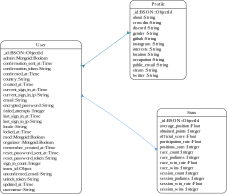
\includegraphics{datamodel1.png}
  \end{center}
  \caption[Modelo de relaciones entre usuario, perfil y estadísticas]{Modelo de relaciones entre usuario, perfil y estadísticas}
  \label{fig:datamodels1}
\end{figure}

\begin{figure}[H]
  \begin{center}
    \includegraphics{datamodel2.png}
  \end{center}
  \caption[Modelo de relación entre temporada, autos y pistas]{Modelo de relación entre temporada, autos y pistas}
  \label{fig:datamodels2}
\end{figure}

\begin{figure}[H]
  \begin{center}
    \includegraphics{datamodel3.png}
  \end{center}
  \caption[Modelo de relaciones entre temporada, ranking y sesiones con sus componentes]{Modelo de relaciones entre temporada, ranking y sesiones con sus componentes}
  \label{fig:datamodels3}
\end{figure}

\begin{figure}[H]
  \begin{center}
    \includegraphics{datamodel4.png}
  \end{center}
  \caption[Modelo de relación entre sesión, carrera y entrada de corredor]{Modelo de relación entre sesión, carrera y entrada de corredor}
  \label{fig:datamodels4}
\end{figure}

\newpage

\section{Esquema de la Base de Datos}
Para facilitar la comprensión de los esquemas de bases de datos presentados a continuación, se ha confeccionado la \autoref{table:schema}, la cual que contiene una pequeña especificación de los atributos utilizados para definir los modelos en el formato de mongoid.

\begin{center}
  \begin{tabular}{ | p{6cm} | p{9cm} |}
    \hline
    \multicolumn{1}{|c|}{\textbf{Atributo}} & \multicolumn{1}{|c|}{\textbf{Detalle}} \\
    \hline
    
    {\textbf{store\_in}} & Declara el nombre de la base de datos de mongo en donde los documentos de este modelo serán almacenados.\\ \hline
    {\textbf{field}} & Declara el nombre de un campo del modelo. \\ \hline
    {\textbf{embeds\_many}} & Declara que el modelo contendrá una colección de modelos anidados. \\ \hline
    {\textbf{accepts\_nested\_attributes\_for}} & Declara que el modelo aceptará atributos para los modelos anidados que éste contenga. \\ \hline
    {\textbf{validates\_presence\_of}} & Valida si el campo proveído no está vacío al momento de guardar el modelo en la base de datos. \\ \hline
    {\textbf{belongs\_to}} & Declara que el modelo tendrá una referencia por ID a otro modelo, quedando esta registrada como un atributo.
    \\ \hline
    {\textbf{has\_many}} & Declara que el modelo podrá ser referenciado por ID desde varios otros modelos. \\ \hline
    {\textbf{has\_one}} & Declara que el modelo contará con una referencia singular por ID a otro modelo. \\ \hline
    {\textbf{validates}} & Declara una o más validaciones para un campo del modelo, tales como su presencia garantizada, singularidad, tamaño mínimo o máximo, entre otras.\\ \hline
  \end{tabular}
  
  \captionof{table}{Tabla de especificación de atributos de esquema de la base datos}\label{table:schema}
\end{center}

Todas las bases de datos dentro de MongoDB están prefijadas utilizando el término ''rv'' (Re-Volt). Por ejemplo, la base de datos que almacena las colecciones de autos se llama ''rv\_cars'', la de los usuarios ''rv\_users'', etc.

A continuación, se exponen fragmentos de código de Ruby con los modelos definidos para este proyecto. Los fragmentos de código están en formato de \textbf{mongoid} (librería de Ruby para MongoDB). Este formato se compone de la declaración de los campos en los modelos mismos, especificando tipo y otras restricciones asociadas. Además, se mezcla el concepto de relaciones entre modelos de Ruby on Rails.

\begin{listing}
  \begin{minted}[mathescape,
    numbersep=5pt,
    frame=single,
    framesep=2mm]{ruby}
class Season
  include Mongoid::Document
  include Mongoid::Timestamps
  include Mongoid::MultiParameterAttributes
  
  store_in :database => 'rv_seasons'
  
  has_many :rankings
  has_many :cars
  has_many :tracks
  
  embeds_many :racer_result_entries
  
  accepts_nested_attributes_for :racer_result_entries
  
  field :name, :type => String
  field :start_date, :type => Date
  field :end_date, :type => Date
  field :current, :type => Boolean, :default => false
  
  validates_presence_of :name
  validates_presence_of :start_date
  validates_presence_of :current
  
  validates_uniqueness_of :name
end
  \end{minted}
\end{listing}

\begin{listing}
  \begin{minted}[mathescape,
    numbersep=5pt,
    gobble=2,
    frame=single,
    framesep=2mm]{ruby}
  class Ranking
    include Mongoid::Document
    include Mongoid::Timestamps
    
    store_in :database => 'rv_rankings'
    
    belongs_to :season
    has_many :sessions
    
    embeds_many :racer_result_entries
    
    accepts_nested_attributes_for :racer_result_entries
    
    field :number, :type => Integer
    
    validates_presence_of :number
  end
  \end{minted}
\end{listing}

\begin{listing}
  \begin{minted}[mathescape,
    numbersep=5pt,
    gobble=2,
    frame=single,
    framesep=2mm]{ruby}
  class Session
    include Mongoid::Document
    include SessionLogUploader::Attachment(:session_log)
    include Mongoid::Timestamps
    
    store_in :database => 'rv_sessions'
    
    belongs_to :ranking
    embeds_many :races
    embeds_many :racer_result_entries
    
    accepts_nested_attributes_for :racer_result_entries
    
    field :number, :type => Integer
    field :host, :type => String
    field :version, :type => String
    field :physics, :type => String
    field :protocol, :type => String
    field :pickups, :type => Boolean
    field :date, :type => Date
    field :teams, :type => Boolean
    field :category, :type => Integer
    field :session_log_data, :type => String
    
    validates_presence_of :number
    validates_presence_of :host
    validates_presence_of :version
    validates_presence_of :physics
    validates_presence_of :protocol
    validates_presence_of :date
    validates_presence_of :session_log
    validates_presence_of :teams
    validates_presence_of :category
  end
  \end{minted}
\end{listing}

\begin{listing}
  \begin{minted}[mathescape,
    numbersep=5pt,
    gobble=2,
    frame=single,
    framesep=2mm]{ruby}
  class User
    include Mongoid::Document
    include Mongoid::Timestamps
    
    store_in :database => 'rv_users'
    
    USERNAME_REGEX = /\A([A-Z0-9_]{1,16}|[0-9a-f]{24})\z/
    
    validates :email, :presence => true, :uniqueness => true
    validates :username, :presence => true, 
    :uniqueness => true, 
    :length => { :minimum => 2, :maximum => 16 }
    validates_format_of :username, :with => USERNAME_REGEX
    
    belongs_to :team, :optional => true
    has_one :team
    
    embeds_one :profile
    embeds_one :stats
    accepts_nested_attributes_for(
    :profile,
    :update_only => true,
    :allow_destroy => false
    )
    accepts_nested_attributes_for(:stats,
    :update_only => true,
    :allow_destroy => false
    )
    
    before_create :create_profile
    before_create :create_stats
    
    field :admin, :type => Boolean, :default => false
    field :mod, :type => Boolean, :default => false
    field :organizer, :type => Boolean, :default => false
    field :locale, :type => String, :default => 'en_us'
    field :country, :type => String
  end
  \end{minted}
\end{listing}

\begin{listing}
  \begin{minted}[mathescape,
    numbersep=5pt,
    gobble=2,
    frame=single,
    framesep=2mm]{ruby}
  class Race
    include Mongoid::Document
    include Mongoid::Attributes::Dynamic
    
    embedded_in :session
    
    embeds_many :racer_entries
    
    field :track_name, :type => String
    field :laps, :type => Integer
    field :racers_count, :type => Integer
    
    validates_presence_of :track_name
    validates_presence_of :laps
    validates_presence_of :racers_count
  end
  \end{minted}
\end{listing}

\begin{listing}
  \begin{minted}[mathescape,
    numbersep=5pt,
    gobble=2,
    frame=single,
    framesep=2mm]{ruby}
  class RacerEntry
    include Mongoid::Document
    include Mongoid::Attributes::Dynamic
    
    embedded_in :race
    
    field :car_name, :type => String
    field :position, :type => Integer
    field :username, :type => String
    field :time, :type => String
    field :best_lap, :type => String
    field :finished, :type => Mongoid::Boolean
    field :cheating, :type => Mongoid::Boolean
    
    validates_presence_of :car_name
    validates_presence_of :position
    validates_presence_of :username
    validates_presence_of :time
    validates_presence_of :best_lap
    validates_presence_of :finished
    validates_presence_of :cheating
  end
  \end{minted}
\end{listing}

\begin{listing}
  \begin{minted}[mathescape,
    numbersep=5pt,
    gobble=2,
    frame=single,
    framesep=2mm]{ruby}
  class Profile
    include Mongoid::Document
    
    embedded_in :user
    
    field :about, :type => String
    field :gender, :type => String
    field :public_email, :type => String
    field :location, :type => String
    field :discord, :type => String
    field :github, :type => String
    field :instagram, :type => String
    field :crowdin, :type => String
    field :steam, :type => String
    field :twitter, :type => String
    field :occupation, :type => String
    field :interests, :type => String
  end
  \end{minted}
\end{listing}

\begin{listing}
  \begin{minted}[mathescape,
    numbersep=5pt,
    gobble=2,
    frame=single,
    framesep=2mm]{ruby}
  class Stats
    include Mongoid::Document
    
    embedded_in :user
    
    field :race_wins, :type => Integer
    field :race_win_rate, :type => Float
    field :race_podiums, :type => Integer
    field :race_count, :type => Integer
    field :positions_sum, :type => Integer
    field :session_wins, :type => Integer
    field :session_win_rate, :type => Float
    field :session_podiums, :type => Integer
    field :session_count, :type => Integer
    field :average_position, :type => Float
    field :participation_rate, :type => Float
    field :official_score, :type => Float
    field :obtained_points, :type => Integer
  end
  \end{minted}
\end{listing}

\begin{listing}
  \begin{minted}[mathescape,
    numbersep=5pt,
    gobble=2,
    frame=single,
    framesep=2mm]{ruby}
  class Car
    include Mongoid::Document
    include Mongoid::Timestamps
    
    store_in :database => 'rv_cars'
    
    belongs_to :season
    
    field :name, :type => String
    field :speed, :type => Float
    field :accel, :type => Float
    field :weight, :type => Float
    field :multiplier, :type => Float
    field :folder_name, :type => String
    field :category, :type => Integer
    field :stock, :type => Boolean, :default => false
    
    validates_presence_of :name
    validates_presence_of :speed
    validates_presence_of :accel
    validates_presence_of :weight
    validates_presence_of :multiplier
    validates_presence_of :folder_name
    validates_presence_of :category
    validates_presence_of :stock
  end
  \end{minted}
\end{listing}

\begin{listing}
  \begin{minted}[mathescape,
    numbersep=5pt,
    gobble=2,
    frame=single,
    framesep=2mm]{ruby}
  class Track
    include Mongoid::Document
    include Mongoid::Timestamps
    
    store_in :database => 'rv_tracks'
    
    belongs_to :season
    
    field :name, :type => String
    field :short_name, :type => String
    field :difficulty, :type => Integer
    field :length, :type => Integer
    field :folder_name, :type => String
    field :stock, :type => Boolean, :default => false
    
    validates_presence_of :name
    validates_presence_of :short_name
    validates_presence_of :difficulty
    validates_presence_of :length
    validates_presence_of :folder_name
    validates_presence_of :stock
  end
  \end{minted}
\end{listing}

\begin{listing}
  \begin{minted}[mathescape,
    numbersep=5pt,
    gobble=2,
    frame=single,
    framesep=2mm]{ruby}
  class RacerResultEntry
    include Mongoid::Document
    
    embedded_in :season
    embedded_in :ranking
    embedded_in :session
    
    field :username, :type => String
    field :country, :type => String
    field :session_count, :type => Integer
    field :race_count, :type => Integer
    field :positions_sum, :type => Integer
    field :average_position, :type => Float
    field :obtained_points, :type => Integer
    field :official_score, :type => Float
    field :participation_multiplier, :type => Float
    field :team, :type => String
    
    validates_presence_of :username
    validates_presence_of :country
  end
  \end{minted}
\end{listing}

\clearpage

\section{Diseño de Interfaz}
El diseño de las interfaces de Re-Volt America ha sido debidamente cuidado al ser implementado en aplicación desarrollada.

En primer lugar, como puede verse en la \autoref{fig:landing}, contamos con una página de inicio con el título de la comunidad de Re-Volt America, junto con varias imágenes del juego para que este pueda ser inmediatamente reconocido por quien visite el portal.

En la parte superior, se encuentra la barra de navegación principal la cual incluye, de izquierda a derecha, los siguientes elementos:
\begin{itemize}
  \item El logotipo de RVA.
  \item Botones para acceder a las secciones más importantes de la web.
  \item Un botón para poder registrarse, iniciar sesión o visualizar información del perfil en caso de existir una sesión iniciada.
\end{itemize}

\begin{figure}[H]
  \begin{center}
    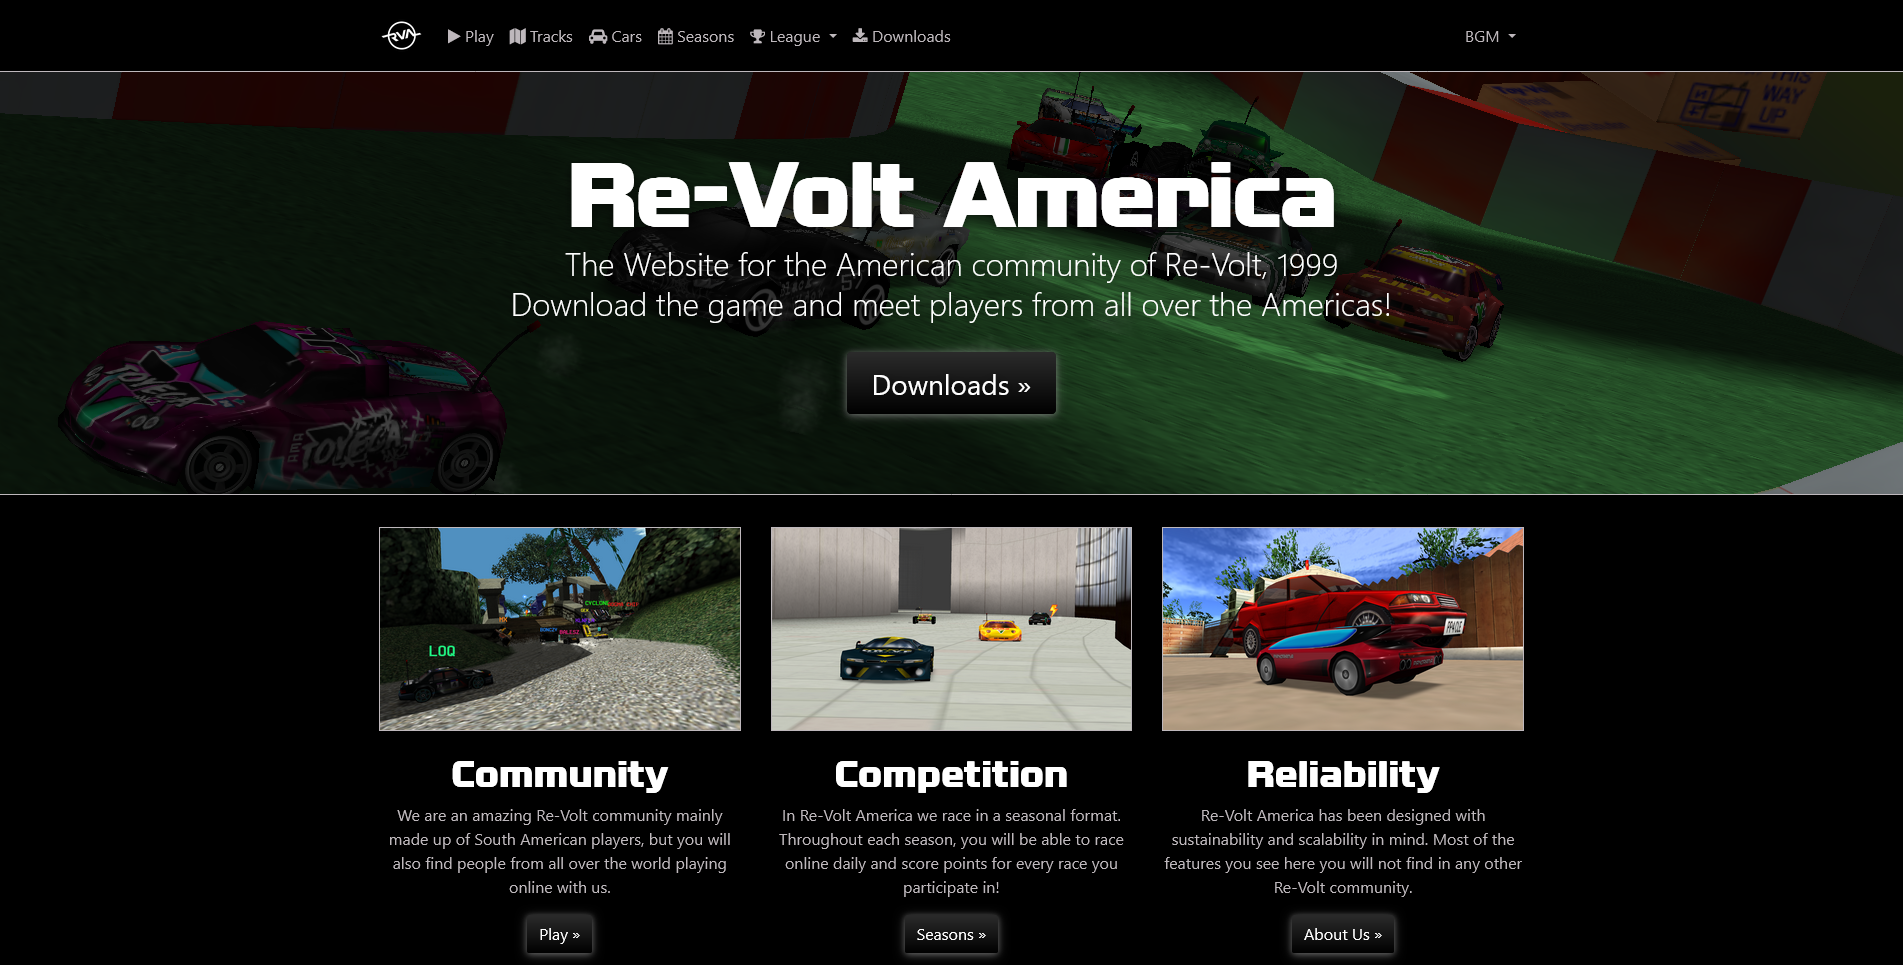
\includegraphics[width=15cm, height=8cm]{img/landing.png} 
  \end{center}
  \caption[Landing page de RVA]{Landing page de RVA}
  \label{fig:landing}
\end{figure}

Dentro de las secciones de autos, pistas y sesiones se cuenta con una barra de sub-navegación, la cual integra todos los elementos de una temporada, dando acceso al usuario de manera más práctica a toda la información que este podría necesitar. El diseño de la interfaz de las sesiones respeta fielmente el formato original de RVA. Estas secciones pueden apreciarse en las \cref{fig:cars,fig:tracks,fig:session}.

\begin{figure}[H]
  \begin{center}
    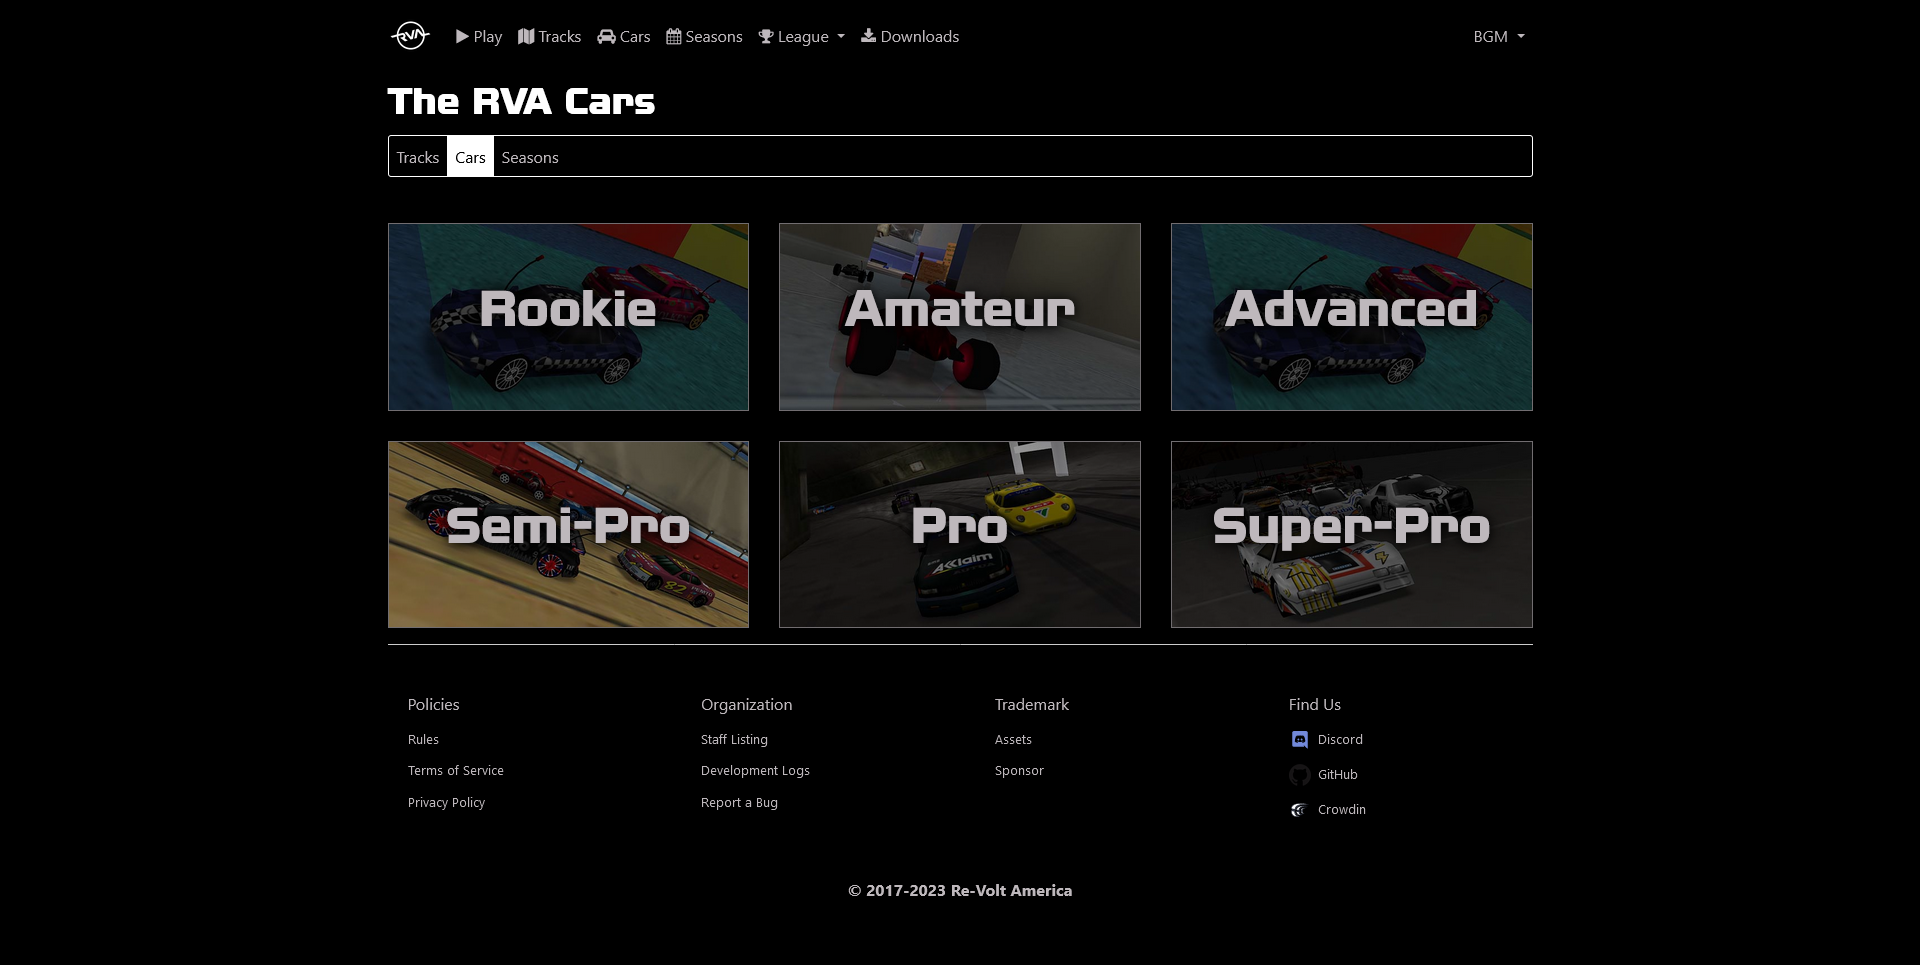
\includegraphics[width=15cm, height=8cm]{img/cars.png} 
  \end{center}
  \caption[Página de autos de RVA]{Página de autos de RVA}
  \label{fig:cars}
\end{figure}

\begin{figure}[H]
  \begin{center}
    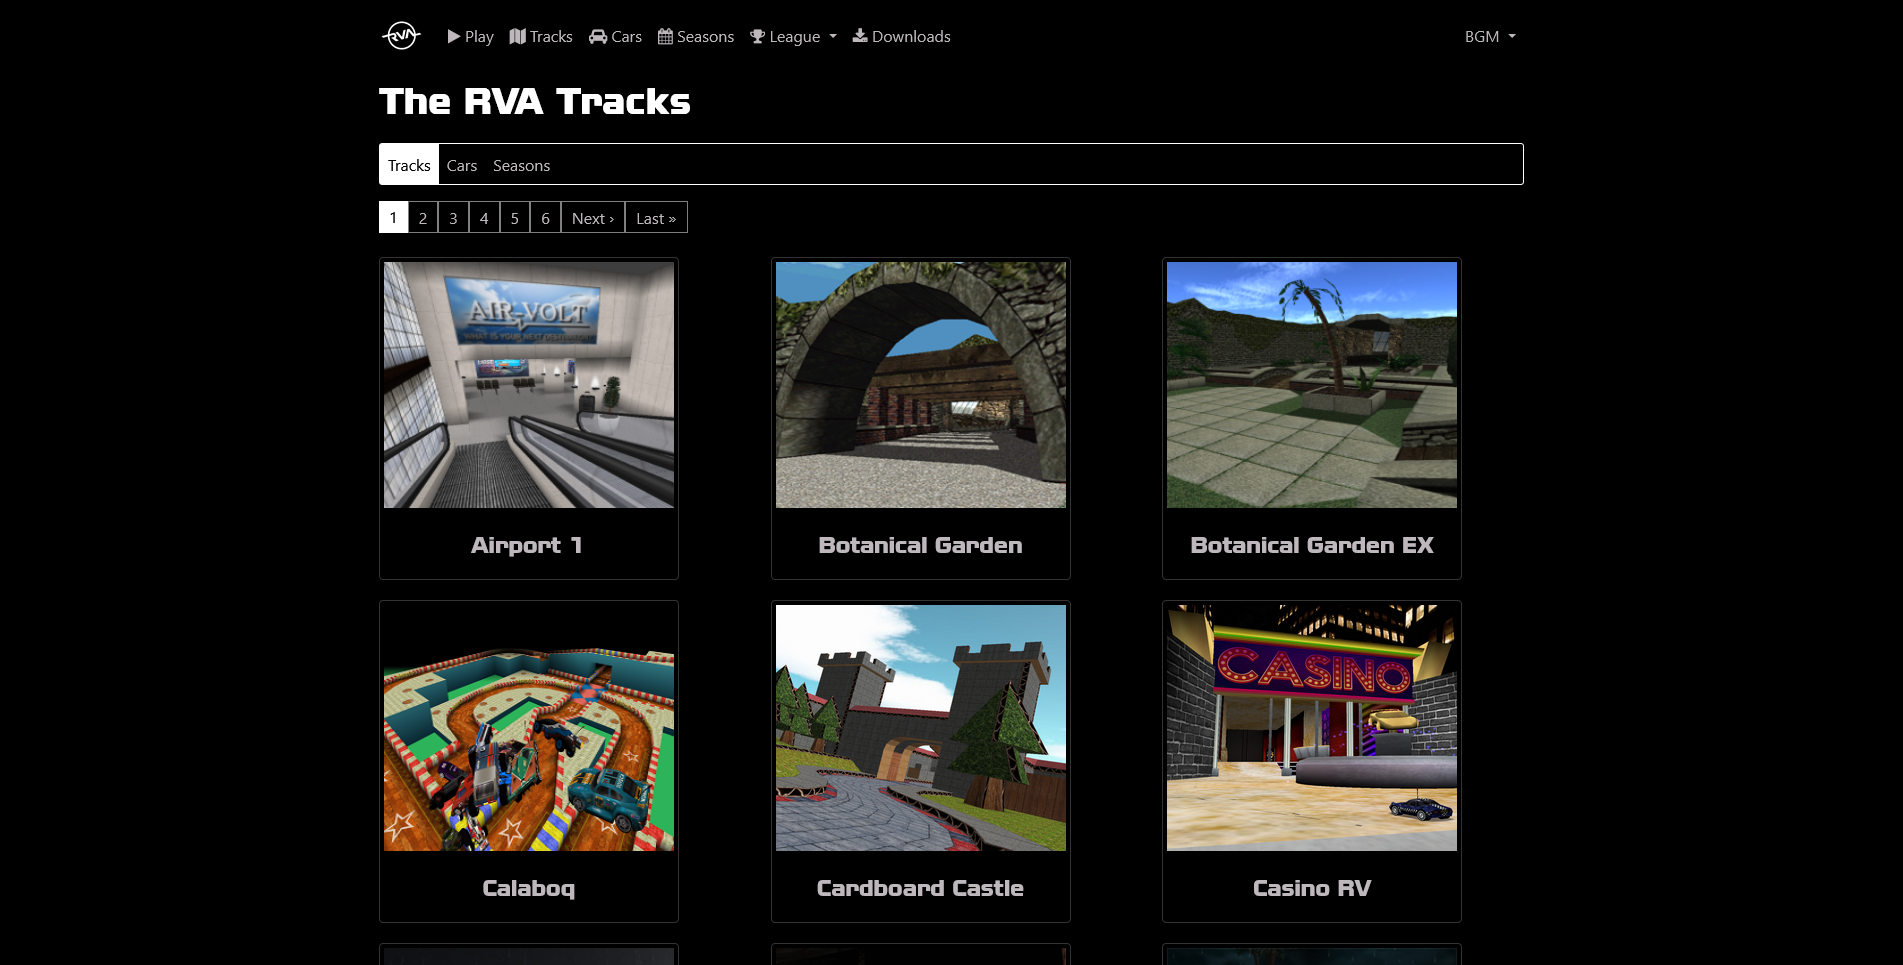
\includegraphics[width=15cm, height=8cm]{img/tracks.png} 
  \end{center}
  \caption[Página de pistas de RVA]{Página de pistas de RVA}
  \label{fig:tracks}
\end{figure}

\begin{figure}[H]
  \begin{center}
    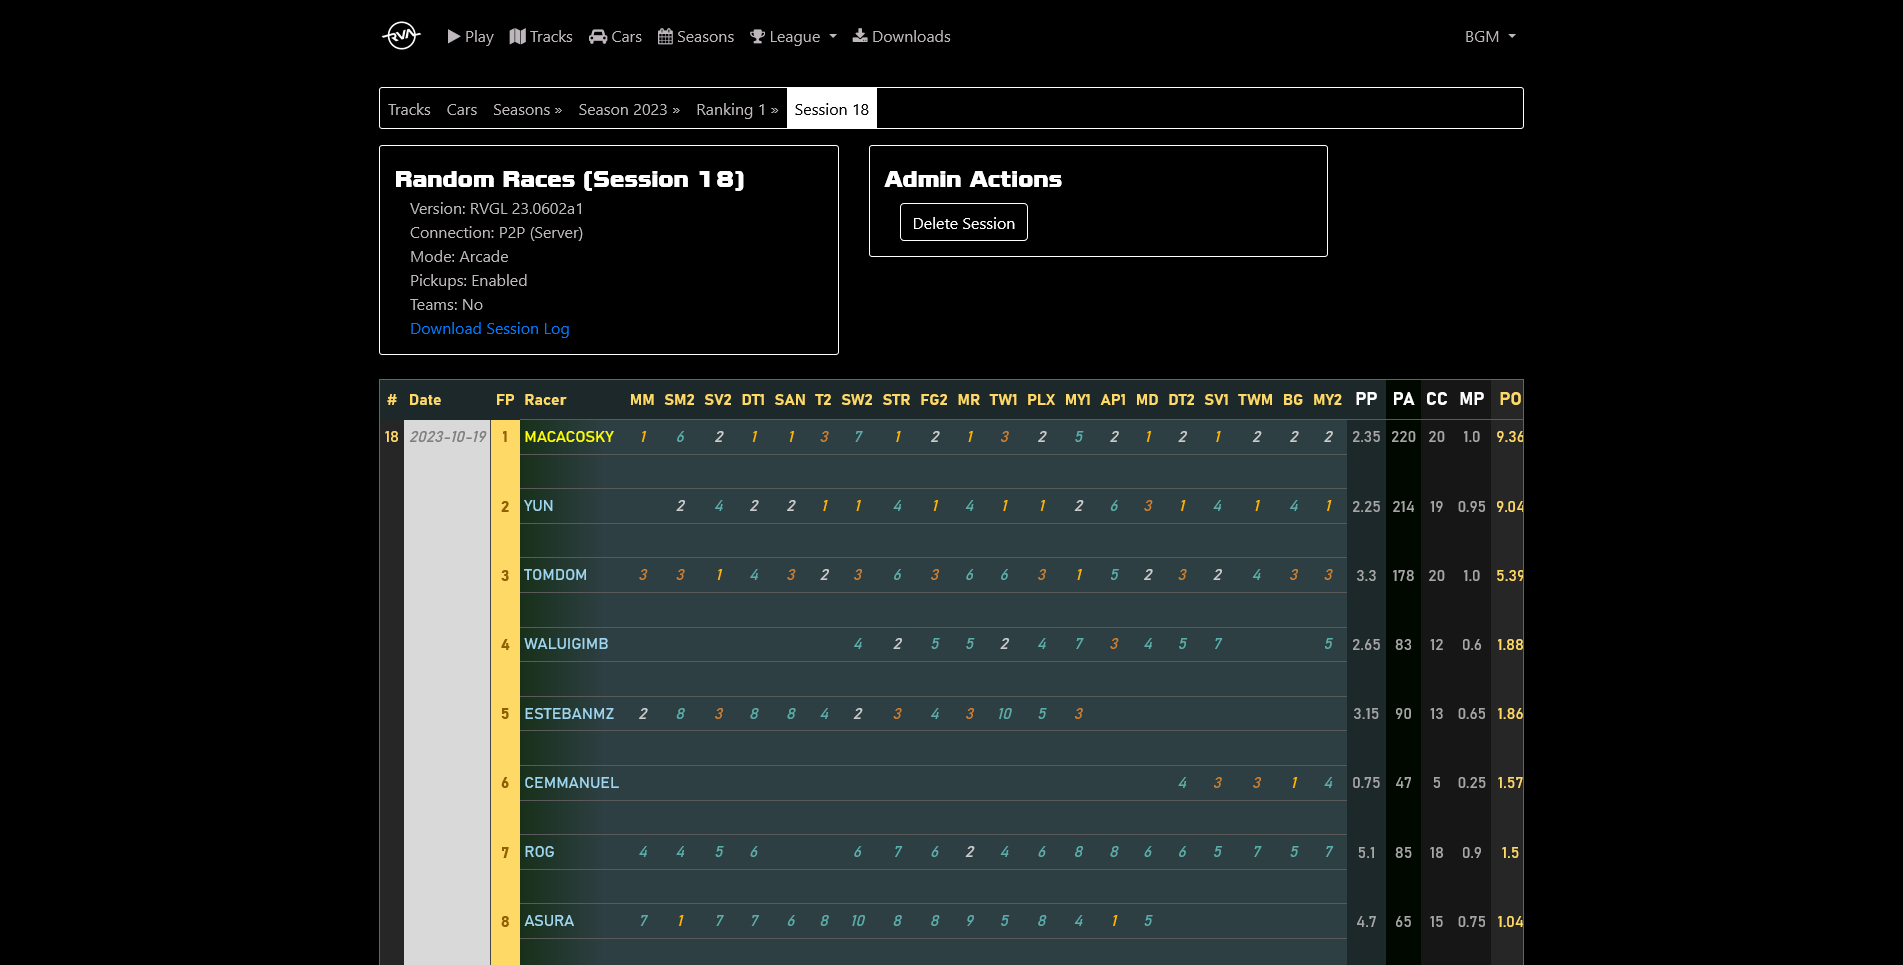
\includegraphics[width=15cm, height=8cm]{img/session.png} 
  \end{center}
  \caption[Página de sesión de RVA]{Página de sesión de RVA}
  \label{fig:session}
\end{figure}

La el diseño de la página de perfil de los usuarios cuenta con su nombre en grande, un resumen de sus estadísticas, posición en el ranking y un pequeño historial de las últimas sesiones en las que han participado, tal como puede verse en la \autoref{fig:profile}.

\begin{figure}[H]
  \begin{center}
    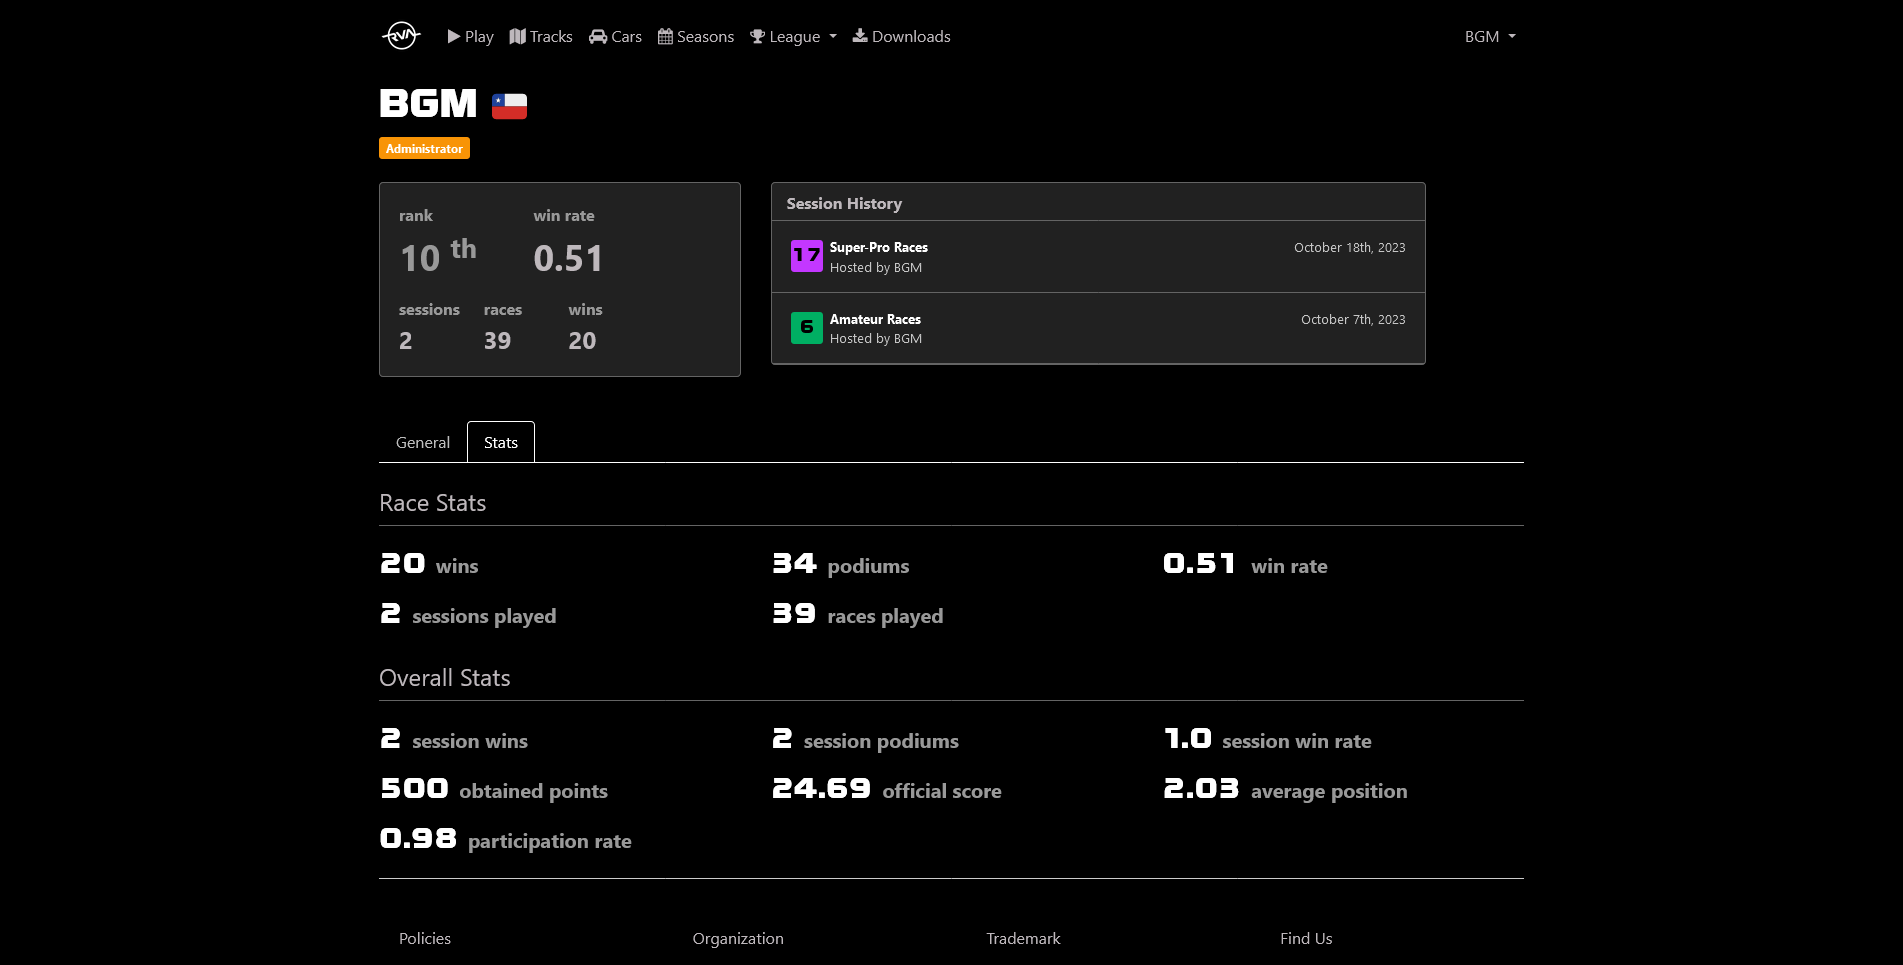
\includegraphics[width=15cm, height=8cm]{img/profile1.png} 
  \end{center}
  \caption[Página de perfil de usuario de RVA]{Página de perfil de usuario de RVA}
  \label{fig:profile}
\end{figure}

Por último, como se muestra en la \autoref{fig:stats}, la página de estadísticas sigue un formato simple de tabla de resultados, con un selector que permite filtrar dichos resultados según diversos criterios.

\begin{figure}[H]
  \begin{center}
    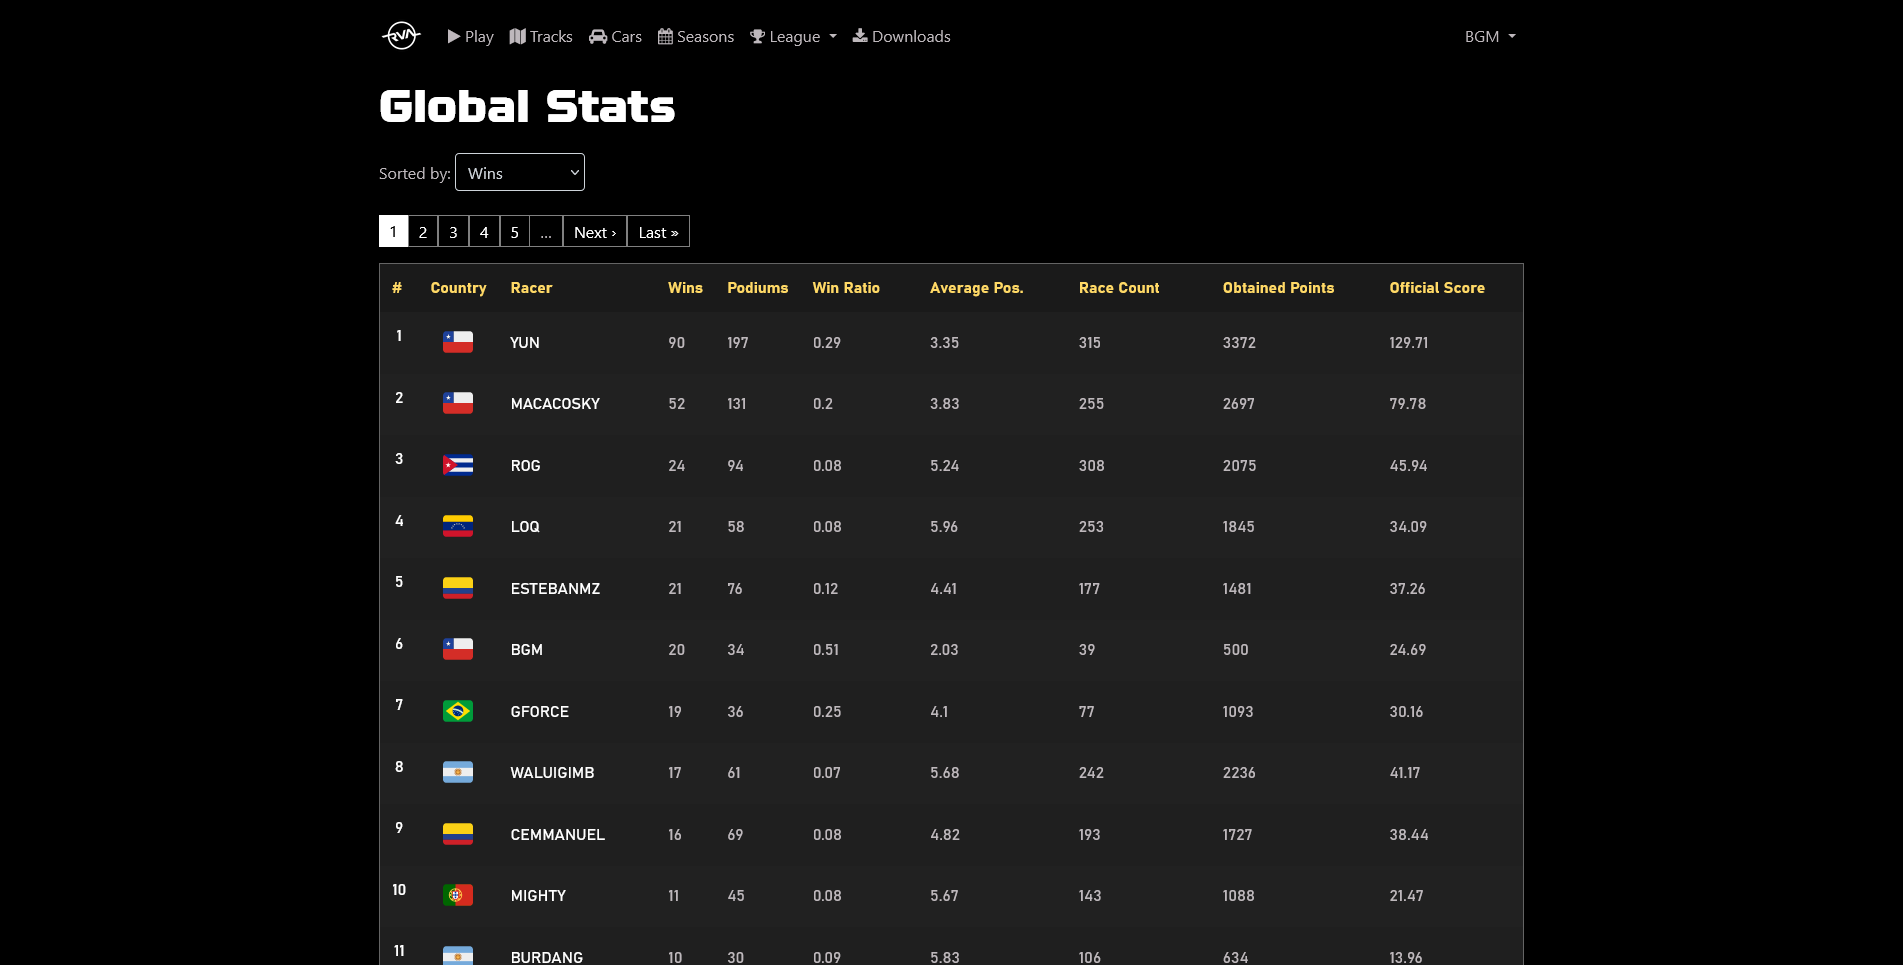
\includegraphics[width=15cm, height=8cm]{img/stats.png} 
  \end{center}
  \caption[Página de estadísticas globales de RVA]{Página de estadísticas globales de RVA}
  \label{fig:stats}
\end{figure}

\subsection{Paleta de Colores y Tipografía}
Como preámbulo principal en cuanto a la paleta de colores y tipografía de RVA, debemos recordar que esta comunidad nace de un grupo de jugadores de Re-Volt, no de una empresa o compañía con estándares definidos. Por lo tanto, para comprender los orígenes de estos elementos, debemos remontarnos a los inicios de Re-Volt America por el año 2017.

Durante los inicios de RVA, se diseña su logo principal, el cual puede apreciarse en la \autoref{fig:rva-logo}.

\begin{figure}[H]
  \begin{center}
    
\includegraphics[width=6cm, height=6cm]{img/rva.png} 
  \end{center}
  \caption[Logotipo de RVA]{Logotipo de RVA}
  \label{fig:rva-logo}
\end{figure}

Del logo de RVA, se derivan los colores blanco y negro (absolutos), los cuales son utilizados como paleta principal para la comunidad.

Así como los colores, la comunidad ha utilizado una fuente muy similar a la de su logotipo a lo largo de los años. Esta fuente se titula ''Nissan Opti'', desarrollada originalmente por Castcraft Software, perteneciente a su marca comercial OptiFont \cite{optifont}. La caracterización de esta compañía tipográfica puede verse a continuación en la \autoref{fig:optifont}.

\begin{figure}[H]
  \begin{center}
    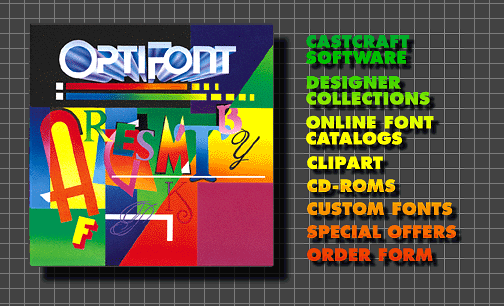
\includegraphics{img/optifont.png} 
  \end{center}
  \caption[Arte de Castcraft Software]{Arte de Castcraft Software}
  \label{fig:optifont}
\end{figure}

De la misma forma, nacen las paletas de colores para las tablas de resultados de sesiones y rankings acumulados, tal como muestran las \cref{fig:session-table,fig:ranking-table}.

\begin{figure}[H]
  \begin{center}
    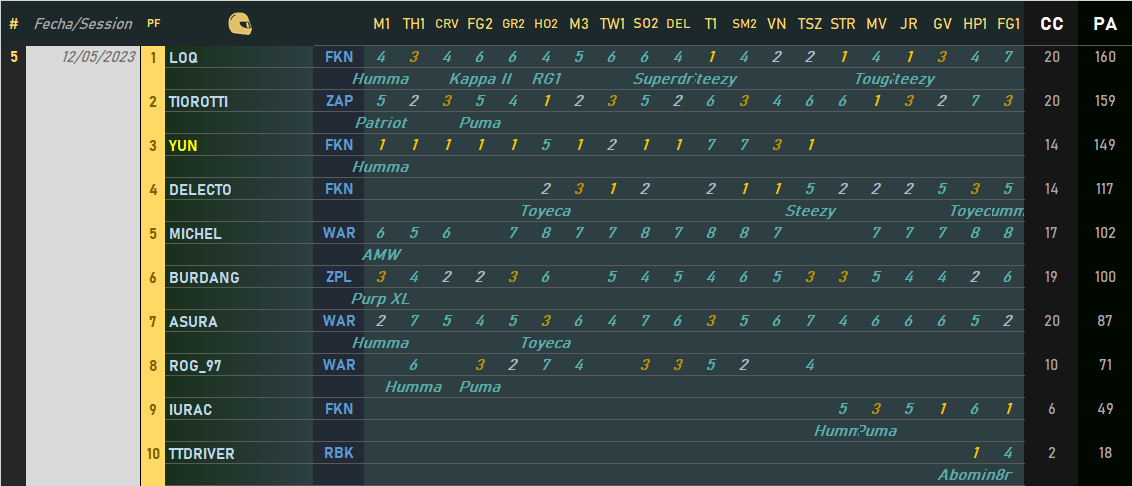
\includegraphics[width=16cm, height=8cm]{img/session_table.png} 
  \end{center}
  \caption[Tabla de resultados de sesión de RVA]{Tabla de resultados de sesión de RVA}
  \label{fig:session-table}
\end{figure}

\begin{figure}[H]
  \begin{center}
    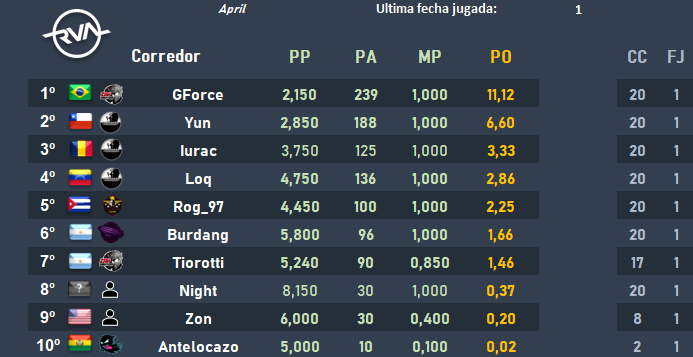
\includegraphics[width=16cm, height=9cm]{img/ranking_table.png} 
  \end{center}
  \caption[Tabla de ranking de RVA]{Tabla de ranking de RVA}
  \label{fig:ranking-table}
\end{figure}

La paleta de colores de las tablas de resultados, junto a su definición en RGB (Red, Green, Blue), puede encontrarse en la \autoref{fig:rva-session-colors} a continuación.

\begin{figure}[H]
  \begin{center}
    \includegraphics[width=15cm, height=10cm]{img/rva_session_colors.png} 
  \end{center}
  \caption[Paleta de colores de sesiones de RVA]{Paleta de colores de sesiones de RVA}
  \label{fig:rva-session-colors}
\end{figure}

\newpage

\section{Diseño de Arquitectura}
El proyecto, en su estado actual, hace uso de un servidor propio, el cual contiene los servicios web, bases de datos y caché. Todo en una sola máquina. Independientemente de donde se termine alojando, la aplicación web estará disponible en ''https://rva.lat/''.

Además de esto, la planificación contempla dos servicios externos, que actualmente son proveídos por GitHub pages \cite{ghpages}, los cuales sirven como repositorios de almacenamiento de datos masivos. Dichos repositorios se encargan, actualmente, de servir información y assets como las imágenes de las pistas y autos que la web ofrece a sus usuarios:

\begin{itemize}
  \item https://tracks.rva.lat/: Repositorio de pistas de RVA.
  \item https://cars.rva.lat/: Repositorio de autos de RVA.
\end{itemize}

A continuación, en la \autoref{fig:architecture}, se muestra un diagrama que ilustra todo el proceso de interacción entre servicios y usuarios.

\begin{figure}[H]
  \begin{center}
    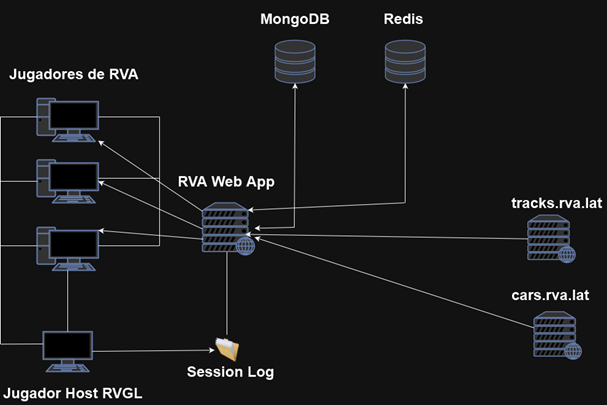
\includegraphics[width=16cm, height=11cm]{img/architecture.png} 
  \end{center}
  \caption[Diagrama de arquitectura de RVA]{Diagrama de arquitectura de RVA}
  \label{fig:architecture}
\end{figure}

Tal como se puede apreciar en la ilustración anterior, la arquitectura que da soporte a la aplicación web de RVA se concentra en un servidor, con dos almacenes de datos. Podemos ver que los usuarios juegan la sesión, el host de la sesión sube el Session Log a la web, y los usuarios pueden visitar la misma web para revisar los resultados.

\newpage

\section{Estructura del Código}
El proyecto, al ser una aplicación hecha en el framework de Ruby on Rails \cite{rubyonrails}, sigue el patrón de MVC (Model View Controller) o modelo, vista, controlador. El árbol de directorios del proyecto se ilustra en la \autoref{fig:tree}.

\begin{figure}[H]
  \begin{center}
    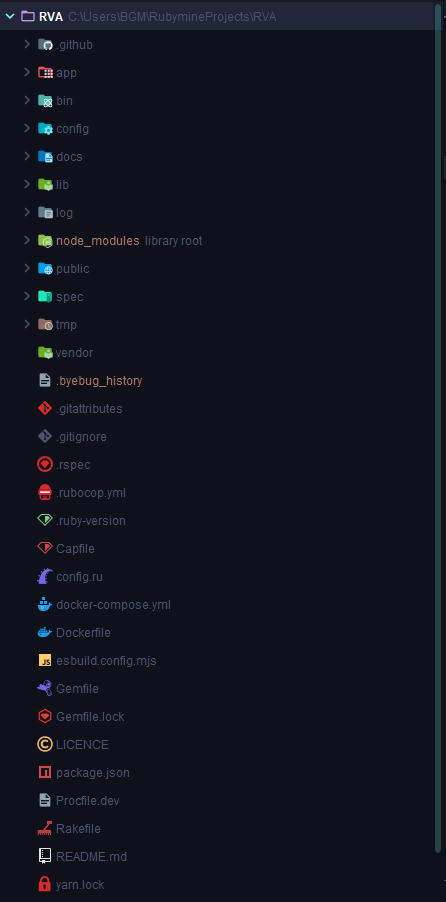
\includegraphics[height=16cm]{img/tree.png} 
  \end{center}
  \caption[Árbol de directorios del proyecto]{Árbol de directorios del proyecto}
  \label{fig:tree}
\end{figure}

Dentro los archivos relevantes para la estructura del código, tenemos aquellos archivos en los que se definen dependencias y módulos de despliegue. La \autoref{table:dependencies} entrega más detalles al respecto.

\begin{center}
  \begin{tabular}{ | l | p{12.5cm} |}
    \hline
    \multicolumn{1}{|c|}{\textbf{Archivo}} & \multicolumn{1}{|c|}{\textbf{Detalle}} \\
    \hline
    
    {\textbf{Capfile}} & Contiene la carga de módulos para el despliegue de la aplicación. \\ \hline
    {\textbf{Gemfile}} & Contiene todas las dependencias del proyecto, con sus respectivas versiones. \\ \hline
  \end{tabular}
  
  \captionof{table}{Tabla archivos de dependencias y módulos de despliegue}\label{table:dependencies}
\end{center}

\subsection{Estándres de Codificación}
El código de este proyecto sigue las recomendaciones estándar para la programación con Ruby, y otros estándares de manera consistente:
\begin{itemize}
  \item Toda la base de código y documentación debe estar escrita en inglés.
  \item Eng eneral, todo el proyecto sigue las convenciones de nombrado y otros lineamientos útiles del sitio de RubyStyle \cite{rubystyle}.
  \item Se utilizan linebreaks (EOL - End of Line) CRLF.
  \item Se utilizan dos espacios para la indentación del código, no tabulaciones.
  \item La codificación del proyecto es en UTF-8. 
\end{itemize}

\subsection{Caché con Redis}
Las llaves o entradas del caché de Redis \cite{redis} son nombradas en minúscula, y los espacios que pudieran existir en ellas son reemplazados por guiones bajos. En caso de llaves compuestas, se utiliza el siguiente formato:

\begin{itemize}
  \item \text{object\_type:id}
  \item \text{object\_type:id\#field}
  \item \text{object\_type:id\#embedded\_object:id}
  \item \text{object\_type:id\#embedded\_object:id\#field}
\end{itemize}

\begin{longlisting}
  \begin{minted}[mathescape,
    linenos,
    numbersep=5pt,
    breaklines,
    frame=single,
    framesep=2mm]{ruby}  
def show
  require 'rva_calculate_results_service'
	
  @count = 0
  @rva_results = Rails.cache.fetch("Session:#{@session.id}") do
    RvaCalculateResultsService.new(@session).call
  end
	
  respond_with @session do |format|
    format.json { render :layout => false }
  end  
end
  \end{minted}
\end{longlisting}


\subsection{Backend}
La \autoref{table:backend} entrega una especificación de los directorios relevantes para el backend del proyecto.

\begin{center}
  \begin{tabular}{ | l | p{12.5cm} |}
    \hline
    \multicolumn{1}{|c|}{\textbf{Directorio}} & \multicolumn{1}{|c|}{\textbf{Detalle}} \\
    \hline
    
    {\textbf{controllers}} & Contiene todos los controladores de Rails, los cuales manejan todas las peticiones web del usuario. \\ \hline
    
    {\textbf{helpers}} & Contiene todas las clases utilitarias, las cuales pueden ser utilizadas para asistir a las clases de modelos, vistas y controladores. \\ \hline
    
    {\textbf{javascript}} & Todo el código de JavaScript utilizado por la aplicación a nivel web se almacena en este directorio.\\ \hline
    
    {\textbf{models}} & Contiene todas las clases que modelan y envuelven los datos almacenados en la base de datos de la aplicación. \\ \hline
    
    {\textbf{services}} & Contiene todas las clases de servicio de la aplicación. Las clases de servicio son aquellos procesos complejos compuestos de mucho código, los cuales se abstraen en servicios para no polucionar los controladores que los requieren. \\ \hline
    
    {\textbf{uploaders}} & Contiene todas las clases relacionadas con la subida de archivos. \\ \hline
    
    {\textbf{config}} & Contiene toda la configuración de la aplicación, como las rutas, inicializadores de librerías, configuración de despliegue, declaración de los entornos de Rails (development, production), configuración de la base de datos y archivos de idioma para la localización del proyecto.\\ \hline
  \end{tabular}
  
  \captionof{table}{Tabla de directorios del backend del proyecto}\label{table:backend}
\end{center}

\subsection{Frontend}
La \autoref{table:frontend} entrega una especificación de los directorios relevantes para el frontend del proyecto.

\begin{center}
  \begin{tabular}{ | l | p{12.5cm} |}
    \hline
    \multicolumn{1}{|c|}{\textbf{Directorio}} & \multicolumn{1}{|c|}{\textbf{Detalle}} \\
    \hline
    
    {\textbf{views}} & Contiene todas las vistas de la aplicación. Todo lo que el usuario ve en la aplicación web tiene su archivo de vista que lo representa. \\ \hline
    
    {\textbf{assets}} & Todas las imágenes, hojas de estilo y demás artefactos requeridos por la aplicación para su correcto funcionamiento y diseño. \\ \hline
    
    {\textbf{public}} & Todos los archivos estáticos servidos por la página pueden encontrarse aquí. Cosas como las páginas de error (404, 422, 500, etc.), estilos compilados, entre otros.\\ \hline
  \end{tabular}
  
  \captionof{table}{Tabla de directorios del frontend del proyecto}\label{table:frontend}
\end{center}
